\documentclass[11pt, a4paper, titlepage]{article}
\usepackage[left=1.5cm,text={18cm, 25cm},top=2.5cm]{geometry}
\usepackage[utf8]{inputenc}
\usepackage[czech]{babel}
\usepackage{hyperref}
\usepackage{amsmath}
\usepackage{graphicx}
\usepackage{wrapfig}
\usepackage{caption}
\usepackage{subcaption} % add sub figures
\usepackage{amsfonts}

% \usepackage{subfig}
% \usepackage{color}
% \usepackage{times}
% \usepackage[bf]{caption}
% \usepackage{hyperref}
% \usepackage[all]{hypcap}
% \usepackage{graphicx}
% \usepackage{url}
% \usepackage[all]{hypcap}
% \hypersetup{colorlinks=false, linkbordercolor=1 1~1, citebordercolor=1 1~1}
% \usepackage[right]{lineno}
% \usepackage{listings}
% \renewcommand\linenumberfont{\normalfont\tiny\color{blue}}

\iflanguage{english}{
    \renewcommand{\uv}[1]{``#1''}
}

% \title{Editory digitální fotografie}
% \subtitle{FYO - Fyzikální optika}
% \author{Petr Fusek <xfusek08@stud.fit.vutbr.cz>}
% \date{\today}


%--------------------------------------------------------------------------------


\begin{document}
\begin{titlepage}
    \begin{center}
        \textsc{\LARGE Fakulta informačních technologií}\\
        \vspace{0.1 cm}
        \textsc{\LARGE Vysoké učení technické v~Brně}\\
        \vspace{\stretch{0.39}}
        {\Huge FYO -- Fyzikální optika}\\
        \vspace{\stretch{0.01}}
        {\huge Editory digitálních fotografií}
        \vspace{\stretch{0.62}}
    \end{center}
    \begin{center}
    \Large
    Petr Fusek \\
    xfusek08@stud.fit.vutbr.cz \\
    \today
    \end{center}
\end{titlepage}


\section{Úvod}
První myšlenka digitální fotografie, byla v~podobě \uv{telefotografie}.
Shelford Bidwell, byl kolem roku 1880 schopen zakódovat obrazové informace pomocí elektrických signálů, které posílal pomocí telegrafu.
Na druhé straně bylo zařízení, které obraz rekonstruovalo řádek po řádku vypalováním obrazových bodů do papíru napuštěného draslíkatým roztokem.
V~roce 1957 Russell Kirsch digitalizoval fotku svého syna a~uložil jí v~malém digitálním souboru na jednom z~raných počítačů.
V~roce 1068 byl sestrojen první senzor, který jako první ukládal světelná data přímo v~digitální podobě, na základě této technologie byla v~roce 1973 postavena první digitální kamera, schopna ukládat obrázky o~rozlišení 0.8 megapixelů.
\cite{first_digital_photography}
 
První veřejně dostupné digitální fotoaparáty se začali objevovat začátkem devadesátých let a~spolu s~nimi výrobci dodávali software, který umožňoval z~fotoaparátu obrázky stáhnout a~dokonce i~upravovat.
První digitální editor ovšem byl součástí digitálního scanneru \uv{Barneyscanner} z~roku 1989, který mohl být použitý k~digitalizaci klasických fotografií a~jejich úpravám.
Tento editor se posléze začal prodávat separátně pod jménem \emph{Adobe Photoshop}.
Photoshop je dnes synonymem pro digitální manipulaci obrázků a~dominuje tento stále rostoucí trh. \cite{digital_editing_histroy}

V~dnešní době jsme si zvykli na základní úpravy obrázků do takové míry, že možnost změnit vlastnosti jako je velikost, jas, kontrast, teplota barev apod., jsou standardem pro jakýkoliv software pracující, nebo jen zobrazující digitální fotografie.
V~této práci se zaměřím na základní teorii a~matematiku schovanou pod některými dobře známými posuvníky.
Například jak a~co je gamma korekce, jak naprogramovat barevný filtr a~jak nejlépe zesvětlit obraz.

\section{Barva a~digitální obraz}
Každý článek o~barvě začíná její definicí jako vjemový zážitek způsobený dopadajícím světlem o~vlnových délkách cca od 400\,nm to 700\,nm, pokračující popisem lidského oka (viz, \cite{wiki:Color},\cite{mul_opora}).
Co je důležité si z~těchto poznatků odnést je, že pořizování, reprezentace v~počítači a~reprodukce barevných obrázků ve všech případech vychází z~toho, jak lidské oko a~mozek reprezentuje barvy.

RGB model, který je používaný v~monitorech pro reprodukci obrazu, je kombinace množství červeného (R), zeleného (G) a~modrého (B) světla, což více méně odpovídá citlivostem 3~barvo-citlivých buněk na sítnici oka.
Na co je ale sítnice nejcitlivější je intenzita dopadajícího světla a~její citlivost se mění pro každou barvu.
Proto intenzita každé složky je nějak empiricky navážena a~manipulace s~nimi či transformace do jiných barevných prostorů jsou otázkou rozsáhlých standardů \cite{wiki:Color_space}.
   
\subsection{Barevné prostory a~modely} \label{color_spaces}
\emph{Barevný prostor} je způsob jakým organizujeme barvy, tak aby jeden bod tohoto prostoru odpovídal jedné konkrétní barvě.
Referenčním standardem je barevný prostor \emph{CIELAB} ($L^*a^*b^*$), který obsahuje všechny barvy, které je lidské oko teoreticky schopno rozeznat \cite{wiki:CIELAB_color_space}.

\emph{Barvený model} je potom matematická abstrakce (množina hodnot), které mapujeme na barevný prostor, který je většinou podmnožinou prostoru referenčního.
Tyto prostory potom slouží jako standard pro kalibraci zobrazovacích a~zaznamenávacích zařízení \cite{wiki:Color_space}.

\subsubsection{RGB}

\begin{wrapfigure}[6]{r}{4.5cm}
    \centering
    \vspace{-1cm}
    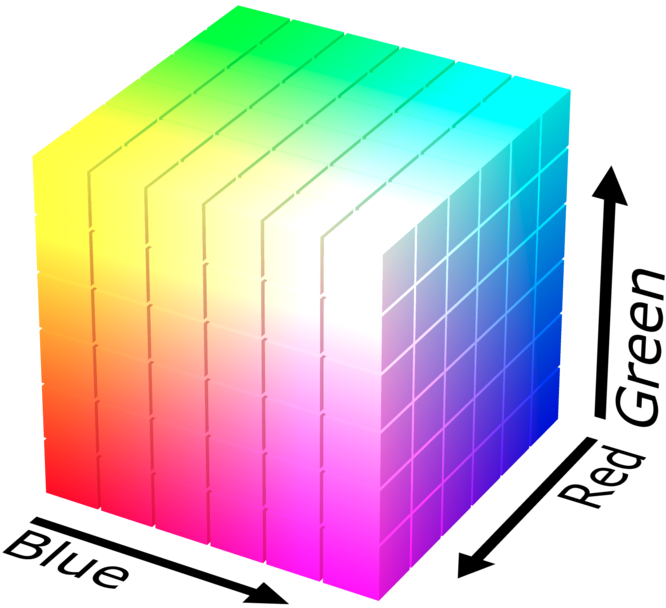
\includegraphics[width=3cm]{RGB_cube.png}
    \caption{RGB prostor \cite{wiki:RGB_color_model}}
\end{wrapfigure}

RGB je asi nejrozšířenější barevný model reprezentovaný jako uspořádaná trojice $(R,G,B)$ hodnot.
Standardizované barevné prostory založené právě na trojicích RGB jsou třeba \emph{Adobe\,RGB}\footnote{\url{https://www.iso.org/standard/45115.html}} nebo \emph{sRGB}\footnote{\url{https://webstore.iec.ch/publication/6169}}.

Popisuje množství světla určitých frekvencí, kterým musí být osvícena sítnice, tak aby jsme jej vnímali jako konkrétní barvu.
Čím více světla (hodnoty) v~každé složce, tím více se blížíme bílé barvě.
Světlo se takto sčítá a~hovoříme o~modelu \emph{aditivním}.


\subsubsection{Y$\text{C}_\text{b}\text{C}_\text{r}$}
\begin{wrapfigure}[12]{r}{5cm}
    \centering
    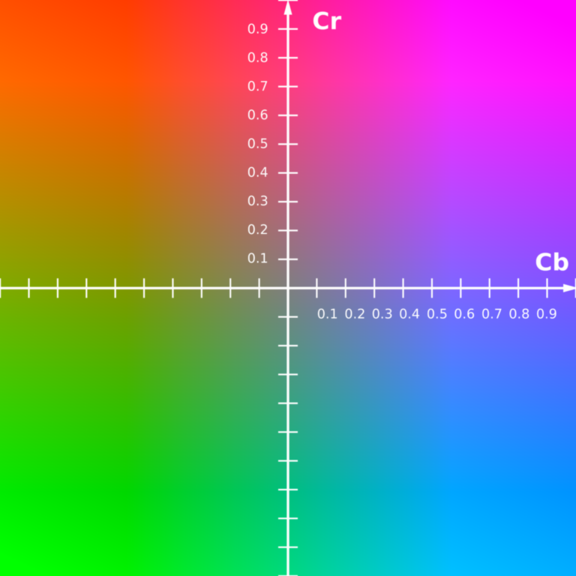
\includegraphics[width=4cm]{YCBCR.png}
    \caption{$\text{C}_\text{b}\text{C}_\text{r}$ výřez při $Y=0.5$ \cite{wiki:YCbCr}.}\label{wrap-fig:1}
\end{wrapfigure}
Model Y$\text{C}_\text{b}\text{C}_\text{r}$ byl vyvinut pro televizní přenosy obrazového signálu, který musel být zpětně kompatibilní s~černobílými televizory.
Využívá právě citlivosti na jas lidského zraku a~většina informací a~detailů je uchována v~jasové Y~složce, čili při zpracování pouze Y~informace dostaneme obraz černobílý.
Složky $\text{C}_\text{b}$ a~$\text{C}_\text{r}$ složí k~posunu jasové informace směrem k~jedné z~barev.
Jasová složka se technicky nazývá \emph{luma} a~z RGB modelu ji lze vypočítat navážením
barvených složek podle empirických citlivostí lidského oka na jednotlivé barvy \cite{mul_opora}:
$$
\begin{bmatrix}Y\\C_b\\C_r\end{bmatrix}
=
\begin{bmatrix}0\\128\\128\end{bmatrix}
+
\begin{bmatrix}
    0,\!299 & 0,\!587 & 0,\!114 \\
    -\,0,\!16875 & -\,0,\!33126 & 0,\!5 \\
    0,\!5 & -\,0,\!41869 & -\,0,\!08131 \\
\end{bmatrix}
\cdot
\begin{bmatrix}R\\G\\B\end{bmatrix}
$$
Výše uvedené koeficienty jsou navrženy pro rychlý přepočet při televizním vysílání, existuje celá škála různých koeficientů pro různé standardy a~formáty s~různými přesnostmi \cite{wiki:YCbCr}.

\subsubsection{HSL a~HSV} \label{hsv/hsl}
HSL a~HSV modely reprezentují intuitivní míchání barev, a~byly vytvořeny, tak aby si uživatel mohl zvolit jak \uv{saturovaná} či jak \uv{světlá} vybraná barva bude.
Prostory jsou v~obou případech válce, kde H~představuje úhel pootočení kolem jeho osy a~tím se zvolí odstín barvy.
S~označuje vzdálenost od osy válce, která symbolizuje saturaci barvy.
L~nebo V~jsou hodnoty jak vysoko se nacházíme s~tím, že L~představuje světlost (maximální L~se rovná bílé) a~V \uv{sílu} zvoleného odstínu (maximální V~je maximálně saturovaná barva) viz obrázek \ref{fig:hsv_hsl}.
\begin{figure}[h]
    \centering
    \begin{subfigure}[b]{0.3\textwidth}
        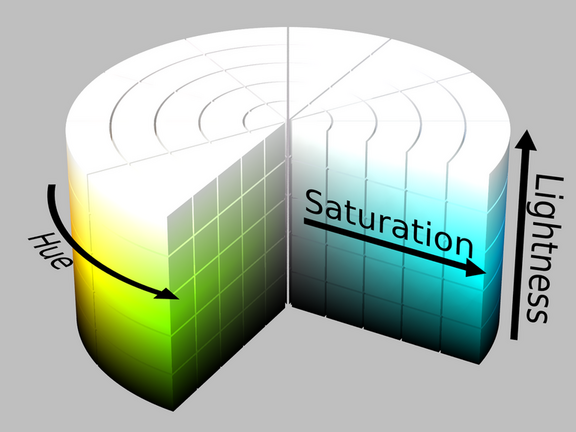
\includegraphics[height=4cm]{HSL.png}
        \caption{$HSL$}
        \label{fig:hsv_hsl:hsl}
    \end{subfigure}
    \hspace{0.2cm}
    \begin{subfigure}[b]{0.3\textwidth}
        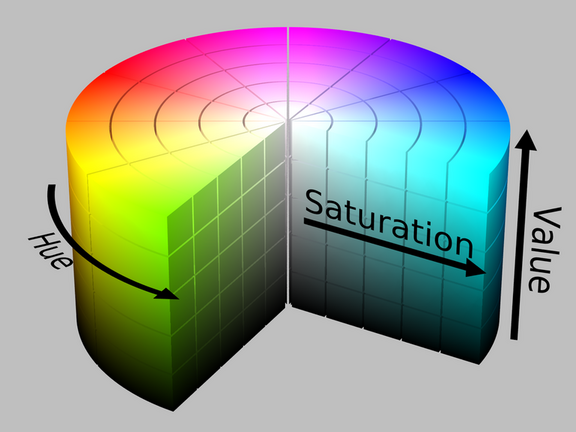
\includegraphics[height=4cm]{HSV.png}
        \caption{$HSV$}
        \label{fig:hsv_hsl:hsv}
    \end{subfigure}
    
    % 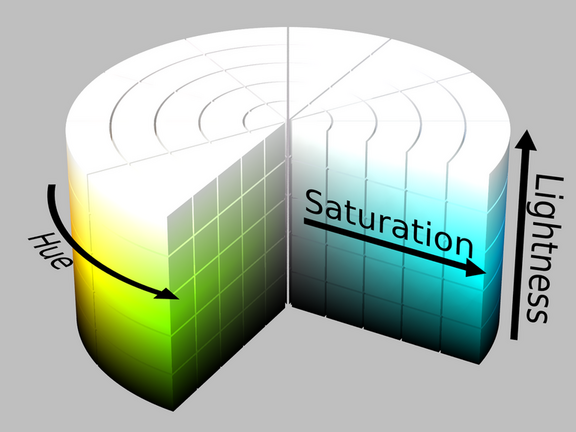
\includegraphics[height=4cm]{HSL.png}
    \caption{Barevné válce \cite{wiki:HSL_and_HSV}}
    
    \label{fig:hsv_hsl}
\end{figure}

\subsection{Reprezentace obrazu v~počítači}
Existuje mnoho způsobů jak ukládat obrazová data v~lineární paměti počítače.
Obrázek je dvourozměrná matice (nebo chcete-li funkce $f(x,y)$), kde jedna hodnota se nazývá pixel (picture element).
Pixely jsou body z~nějakého barevného modelu (viz. \ref{color_spaces}), nejčastěji RGB, tedy 3~hodnoty, kde $(0,0,0)$ udává barvu černou a~$(\text{\small MAX}, \text{\small MAX}, \text{\small MAX})$ barvu bílou.
Jednotlivé barevné složky se nazývají subpixely a~jejich hodnota \uv{$\text{\small MAX}$} je dána počtem bytů, na kterém složky chceme reprezentovat.
Hodnotám subpixelů je nejčastěji rezervován jeden bajt (8 bitů) čili celočíselné hodnoty z~intervalu $\langle0;255\rangle$.
Vzniká tak prostor čítající $256^3 = 16\,777\,216$ možných barev, což je pro běžného člověka dostatečné množství.
Pokud jsou jednotlivé hodnoty v~pamětu uloženy těsně za sebou v~pořadí R-G-B, vychází na jeden pixel 24 bitů a~značíme jej jako pixel o~formátu RGB24.
Existuje celá řada formátů jejichž označení vypovídá o~jejich rozložení a~velikosti v~paměti (RGB555, BRG24, RGBA32\footnote{A složka označuje alfa kanál, který přižazuje míru průhlednosti pixelu.}, ...) \cite{mul_opora}.

Takto nekomprimovaná obrazová data jsou v~sérii pixel po pixelu uloženy v~paměti nazývané \emph{framebuffer}.
Obrázek má definovaný počet sloupců a~počet řádků.
Jsou očekávávatelně sekvence pixelů jdoucí za sebou, ale v~paměti mohou být řádky uspořádané shora dolů nebo zespodu nahoru.
Mezi řádky se rovněž vkládá \emph{padding}, tak aby jejich začátky byly zarovnané a~adresovatelné pro rychlejší přístup k~paměti (rozložení můžete vidět na obrázku \ref{fig:framebuffer}).

\begin{figure}[h]
    \centering
    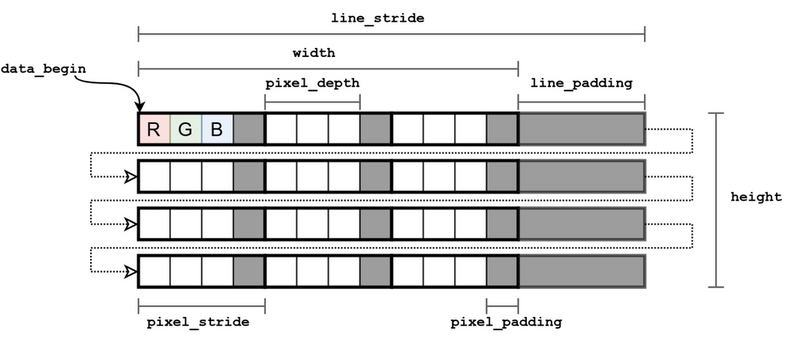
\includegraphics[width=0.9\textwidth]{framebuffer.png}
    \caption{Rozložení framebuffer v~paměti \cite{Whatdoes20:online}}
    \label{fig:framebuffer}
\end{figure}

S~takto uloženými daty je možno libovolně manipulovat a~zobrazovat je uživateli.
Pro jejich ukládání se volí různé kompresní formáty, které jsou mimo záběr této práce.
Editor ovšem musí vždy takový komprimovaný obrázek umět načíst ze souboru do nekomprimovaného framebufferu a~po provedených změnách jej v~komprimované podobě zase uložit. Velkost nekomprimovaného  framebufferu je z~pravidla řádově větší než velikost komprimovaných dat.
Nejpoužívanějším formátem pro ukládání fotografií je \emph{JPEG}, který provádí ztrátovou kompresi a~pro bezztrátovou kompresi obrázků s~omezenou paletou barev se využívá například formát \emph{PNG}.

% \section{Operace nad obrázky}
% Tato sekce je zaměřena na různé operace, které se s~pixely ve framebufferu nejčastěji provádějí, otevře-li uživatel libovolný editační nástroj.
% Pro jednoduchost v základu pracujeme s modelem, kde pixel $P$ reprezentujeme takto:
% $$P = (r,g,b)$$
% Jednotlivé složky $r$, $g$ a $b$ jsou reálná čísla z intervalu $\langle0,1\rangle$.
% Tato reprezentace se vždy implicitně po provedení výpočtu namapuje na RGB24 model, který lze značit takto:
% $$P_i=(R,G,B) \quad \text{, kde }(R,G,B) \in [\![0\,..\,255]\!]^3$$
% Převod z $P$ na $P_i$ je definován po složkách:
% $$p_i=\left\lfloor 255p+\dfrac{1}{2}\right\rfloor$$

% \newpage
% \subsection{Expozice}
% Korekce jasu je ve většině editorech nazývaná \uv{expozice} a většinou je implementována velice triviálním způsobem pomocí přičtení hodnoty $\delta$ ke každému subpixelu.
% $$
% P' =
% \begin{bmatrix}
%     crop(r+\delta, 0, 1) \\
%     crop(g+\delta, 0, 1) \\
%     crop(b+\delta, 0, 1)
% \end{bmatrix}
% \quad
% \text{, kde }\delta \in \langle-1,1\rangle
% $$
% \subsection{Gamma}
% Tato operace je nelineární transformací, kde dochází ke změně dynamického rozsahu pomocí mocnění hodnoty jasu. (Luma složky) na hodnotu $\gamma$ \cite{wiki:Gamma_correction}.
% $$(Y, C_b, C_r) = to\_YC_bC_r(r,g,b)$$
% $$P' = to\_RGB(Y^\gamma, C_b, C_r)$$

% \subsection{Kontrast}
% Kontrastem rozumíme změnu rozdílu
% \subsection{Teplota barvy}
% \subsection{Tónování}
% \subsection{Rozmazání a~Filtrace}
\section{Implementace}
V rámci práce byl implementován jednoduchý editor, který demonstruje možnosti základních filtrovacích operací/transformací nad daty nahraného obrázku.

K implementaci byl použit programovací jazyk rust\footnote{\url{https://www.rust-lang.org/}} s knihovnou \texttt{egui}\footnote{\url{https://github.com/emilk/egui}} pro implementaci aplikací s grafickým uživatelským rozhraním.
Díky těmto technologiím lze aplikaci přeložit téměř pro všechny platformy podporující grafické rozhraní \texttt{OpenGL}\footnote{\url{https://www.opengl.org/}}.
\subsection{Implementované operace}
Aplikace funguje tak, že po spuštění se objeví uvítací obrazovka, která vyzve uživatele aby vybral obrázek ze svého počítače. Poté mu je umožněno aplikovat sérii filtrů, které jsou popsány níže.
Hlavní obrazovka editoru je vidět na obrázku \ref{fig:screenshot}.
\begin{figure}[h]
    \centering
    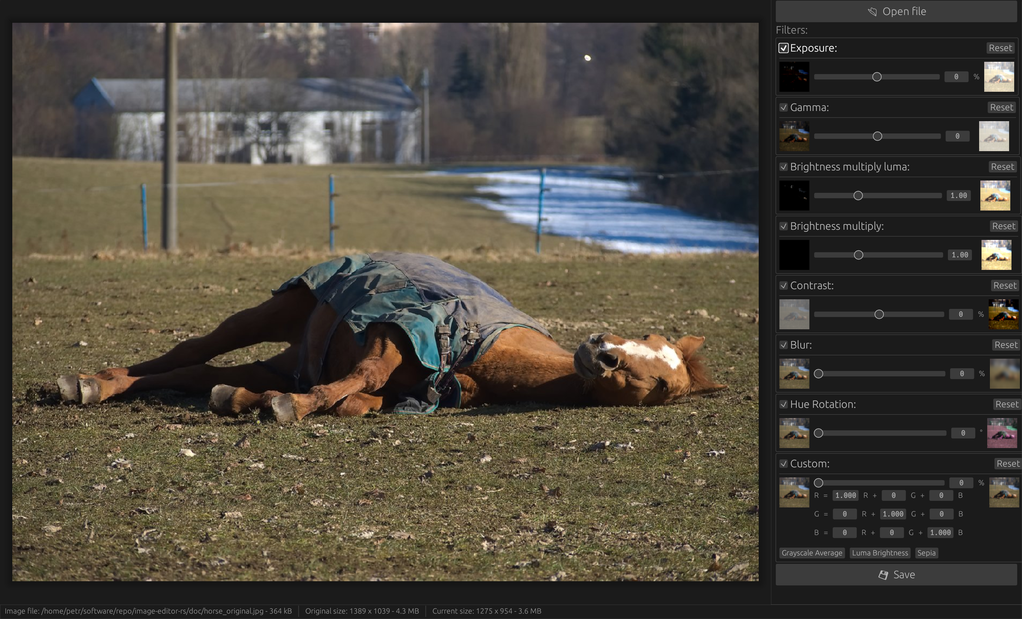
\includegraphics[width=0.9\textwidth]{screenshot.png}
    \caption{Snímek hlavní obrazovky editoru}
    \label{fig:screenshot}
\end{figure}

\subsubsection{Expozice}
Nejjednodušším filtrem je expozice, která je součástí každého editoru.
její implementace spočívá v přičtení konstantní hodnoty ke všem subpixelům.
$$P' = \delta + P$$
Na obrázku \ref{fig:exposure} je vidět přitení záporné hodnoty pro ztmavení a kladné pro zesvětlení.
\begin{figure}[h]
    \centering
    \begin{subfigure}[t]{0.25\textwidth}
        \vskip 0pt
        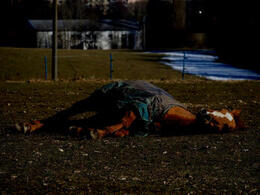
\includegraphics[width=1.0\textwidth]{horse_exposure_minus.jpg}
        \caption{Záporná expozice - ztmavení obrázku}
    \end{subfigure}
    \hspace{1cm}
    \begin{subfigure}[t]{0.25\textwidth}
        \vskip 0pt
        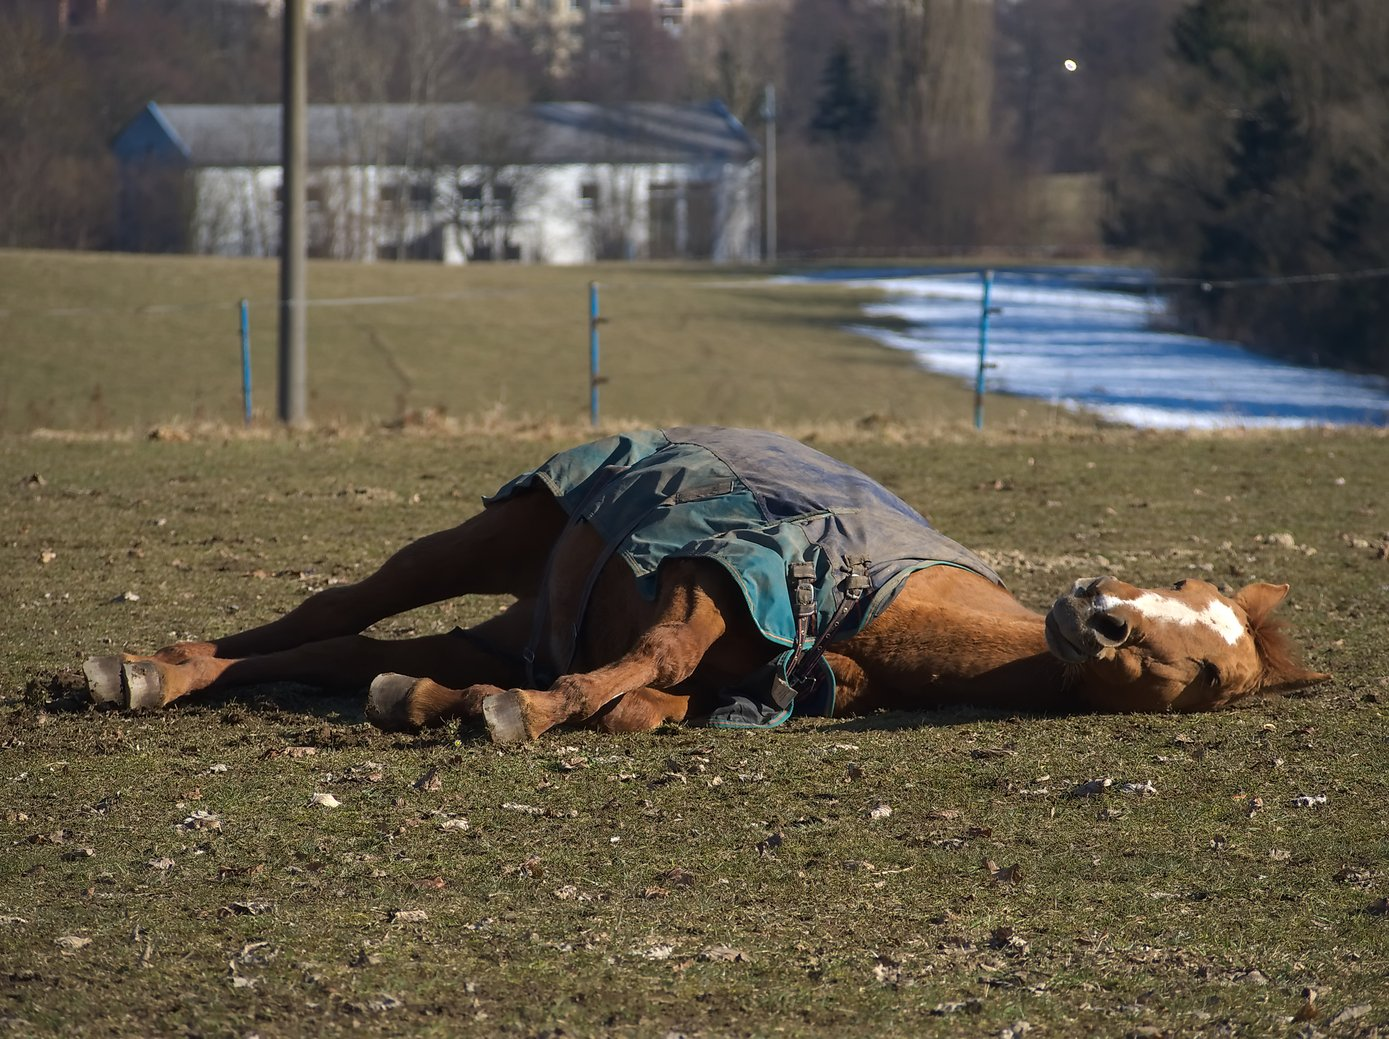
\includegraphics[width=1.0\textwidth]{horse_original.jpg}
        \caption{Původní obrázek}
    \end{subfigure}
    \hspace{1cm}
    \begin{subfigure}[t]{0.25\textwidth}
        \vskip 0pt
        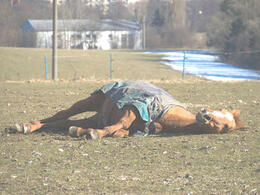
\includegraphics[width=1.0\textwidth]{horse_exposure_plus.jpg}
        \caption{Kladná expozice - zesvětlení obrázku}
    \end{subfigure}
    \caption{Výsledky operace \uv{Expozice}}
    \label{fig:exposure}
\end{figure}
Zde je vidět, že efekt není příliš šetrný a způsobuje bílou mlhu a nezachovává stíny.

\subsubsection{Gamma}
Gamma korekce je nelineární transformace pracující s jasovou složkou obrázku.
Počítá se umocněním jasu na hodnotu $\gamma \leq 0$ \cite{wiki:Gamma_correction}.
$$V_{out}=V_{in}^\gamma$$
Pokud $\gamma < 1.0$ tmavší pixely budou zesvětleny a čím více pixel světlejší je, tím méně bude ovlivněn.
Při $\gamma > 1.0$ budou hodnoty tmavších pixelů zredukovány a zvýší se tak kontrast světlé vůči tmavé.
Výsledek této operace je vidět na obrázku \ref{fig:gamma}.
\begin{figure}[h]
    \centering
    \begin{subfigure}[t]{0.25\textwidth}
        \vskip 0pt
        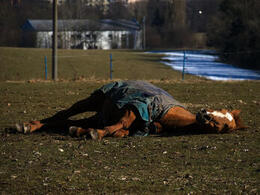
\includegraphics[width=1.0\textwidth]{horse_gamma_minus.jpg}
        \caption{Obrázek pro $\gamma = 0.5$}
    \end{subfigure}
    \hspace{1cm}
    \begin{subfigure}[t]{0.25\textwidth}
        \vskip 0pt
        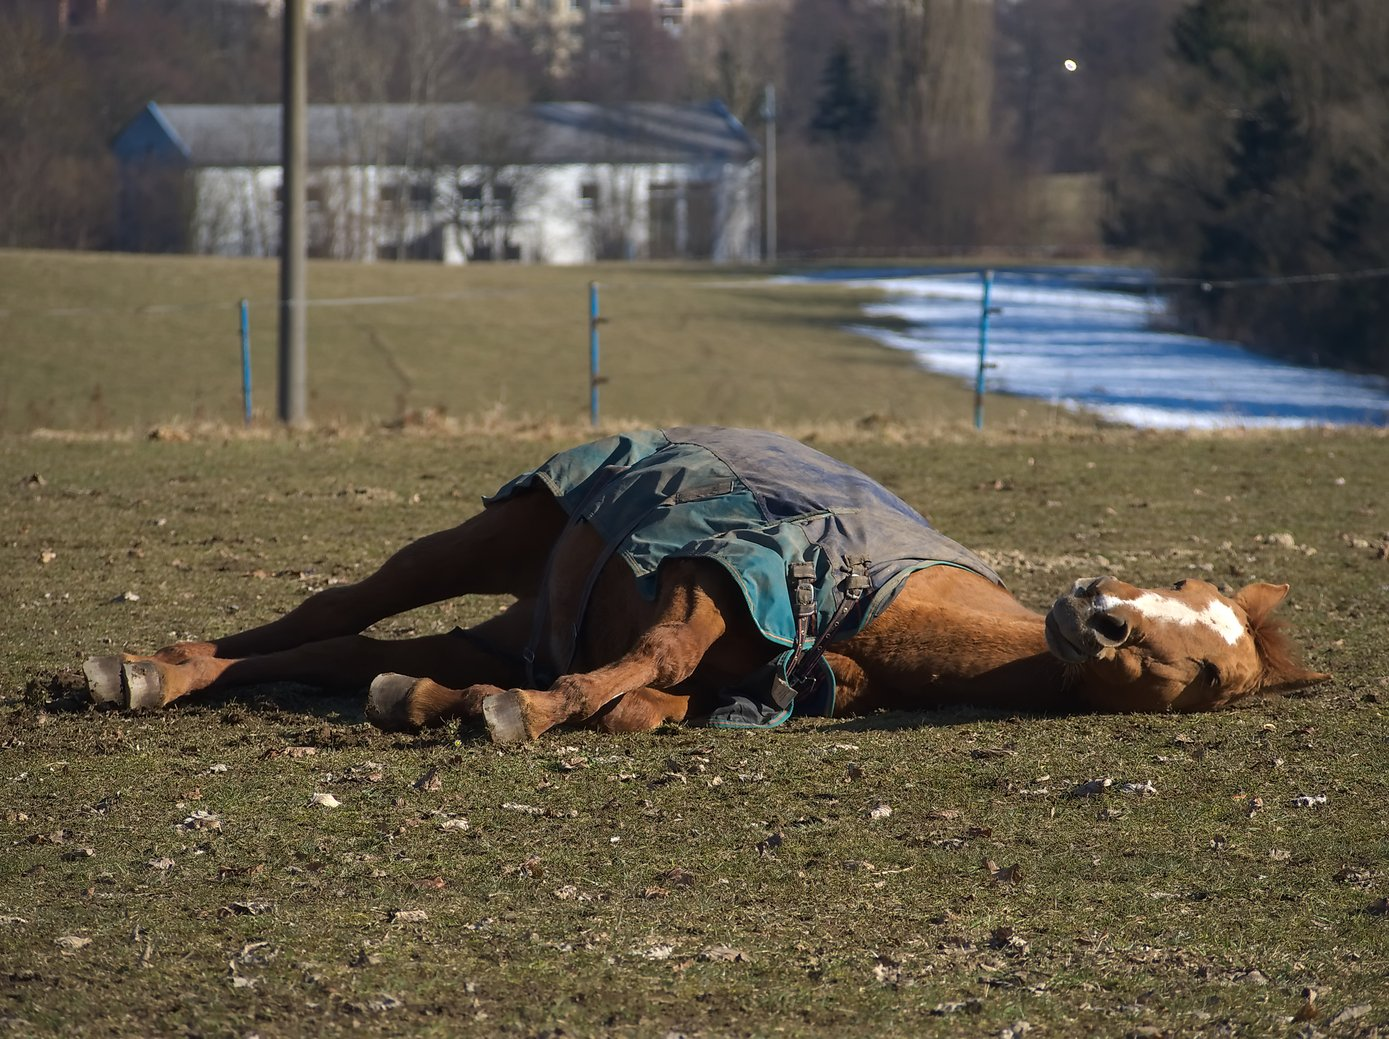
\includegraphics[width=1.0\textwidth]{horse_original.jpg}
        \caption{Původní obrázek ($\gamma = 1$)}
    \end{subfigure}
    \hspace{1cm}
    \begin{subfigure}[t]{0.25\textwidth}
        \vskip 0pt
        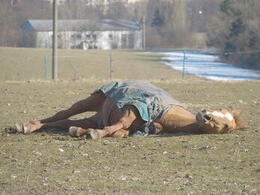
\includegraphics[width=1.0\textwidth]{horse_gamma_plus.jpg}
        \caption{Obrázek pro $\gamma = 1.5$}
    \end{subfigure}
    \caption{Výsledky operace \uv{Gamma}}
    \label{fig:gamma}
\end{figure}
Oproti jednoduché expozici bílá mlha není tak nápadná a ztmavení se jeví více vyrovnaným dojmem.

\subsubsection{Kontrast}
Úprava kontrastu znamená, že měníme relativní rozdíl barvy a jasu pixelu oproti středí hodnotě celého obrázku \cite{wiki:Contrast_vision}.
Současná implementace je v tomto případě záležitostí použité knihovny \texttt{image}\footnote{\url{https://github.com/image-rs/image}}.
Výsledek je vidět na obrázku \ref{fig:contrast};
\begin{figure}[h]
    \centering
    \begin{subfigure}[t]{0.25\textwidth}
        \vskip 0pt
        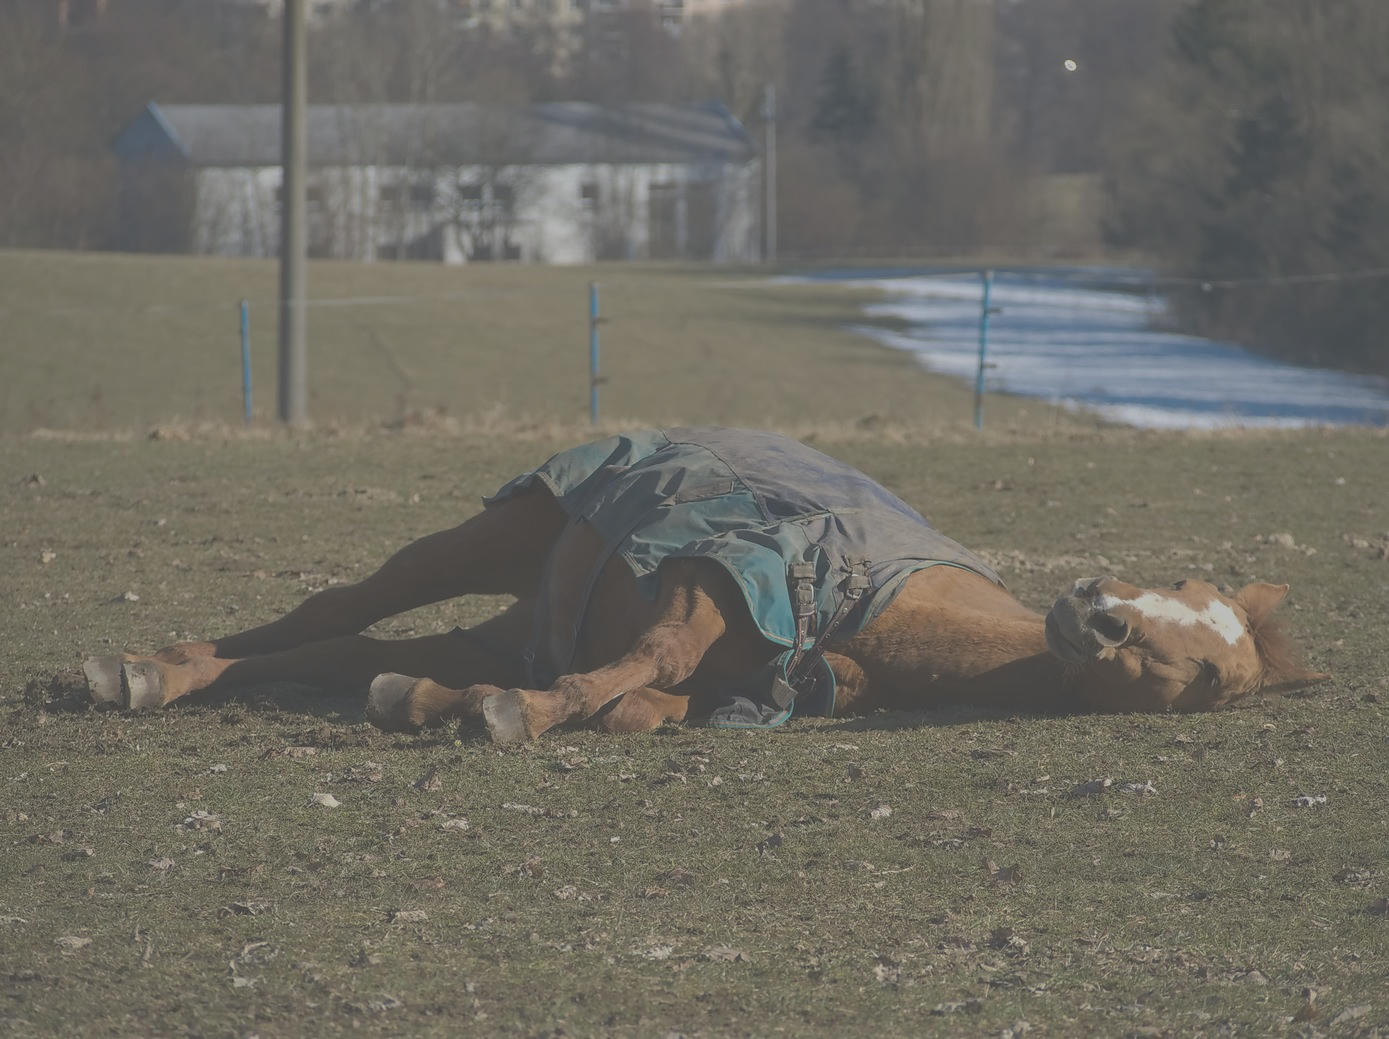
\includegraphics[width=1.0\textwidth]{horse_contrast_minus.jpg}
        \caption{Snížený o 50\%}
    \end{subfigure}
    \hspace{1cm}
    \begin{subfigure}[t]{0.25\textwidth}
        \vskip 0pt
        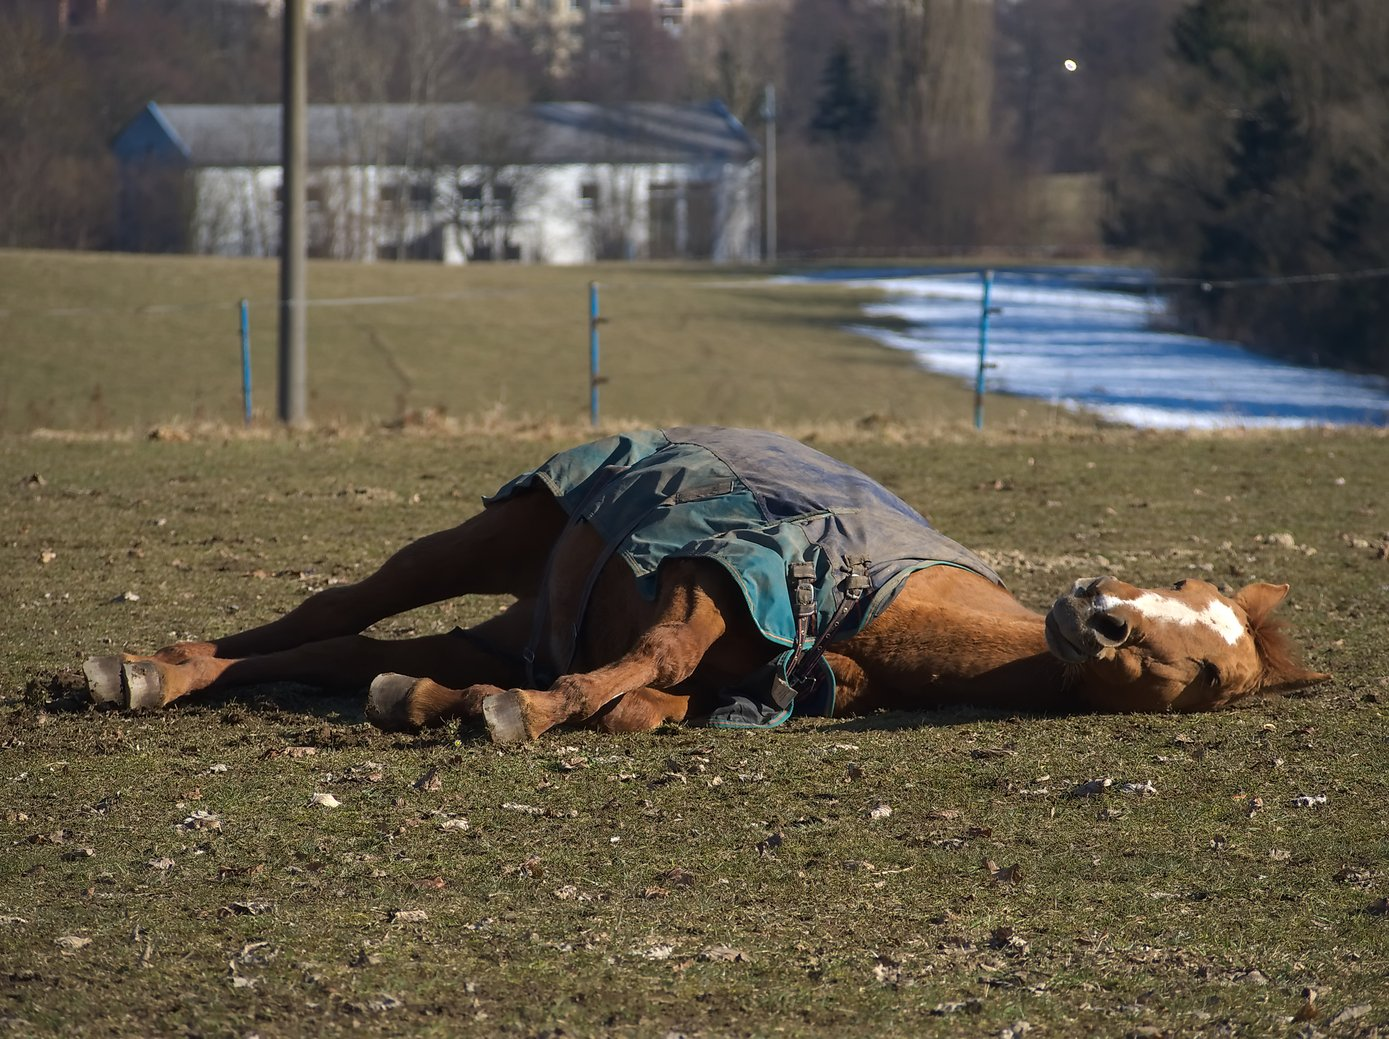
\includegraphics[width=1.0\textwidth]{horse_original.jpg}
        \caption{Původní obrázek.}
    \end{subfigure}
    \hspace{1cm}
    \begin{subfigure}[t]{0.25\textwidth}
        \vskip 0pt
        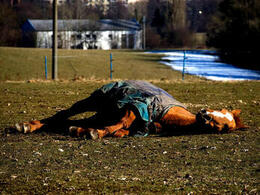
\includegraphics[width=1.0\textwidth]{horse_contrast_plus.jpg}
        \caption{Zvýšený o 50\%}
    \end{subfigure}
    \caption{Výsledky operace úpravy kontrastu}
    \label{fig:contrast}
\end{figure}


\subsubsection{Rozmazání}
Efekt rozmazání se docílí pomocí zprůměrování hodnot současného okolních pixelů.
Současná implementace je v tomto případě záležitostí použité knihovny \texttt{image}.
\begin{figure}[h]
    \centering
    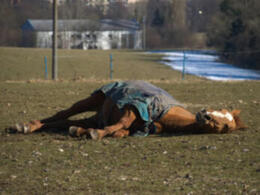
\includegraphics[height=5cm]{horse_blur.jpg}
    \caption{Maximální rozmazání, které aplikace dovoluje.}
    \label{fig:blur}
\end{figure}

\subsubsection{Rotace odstínu}
Tato operace pracuje s HSV nebo HSL barevným prostorem \ref{hsv/hsl}.
Každý pixel obrázku se převede do odpovídající HSL / HSV reprezentace a upraví se hodnota H (hue).
Tato hodnota udává velikost úhlu otočení kolem osy barevného válce, je tedy periodická a nabývá hodnoty 0 až $360^\circ$.
Hodnoty podle úhlu jsou znázorněny na obrázku \ref{fig:huerotate-scale}.
\begin{figure}[h]
    \centering
    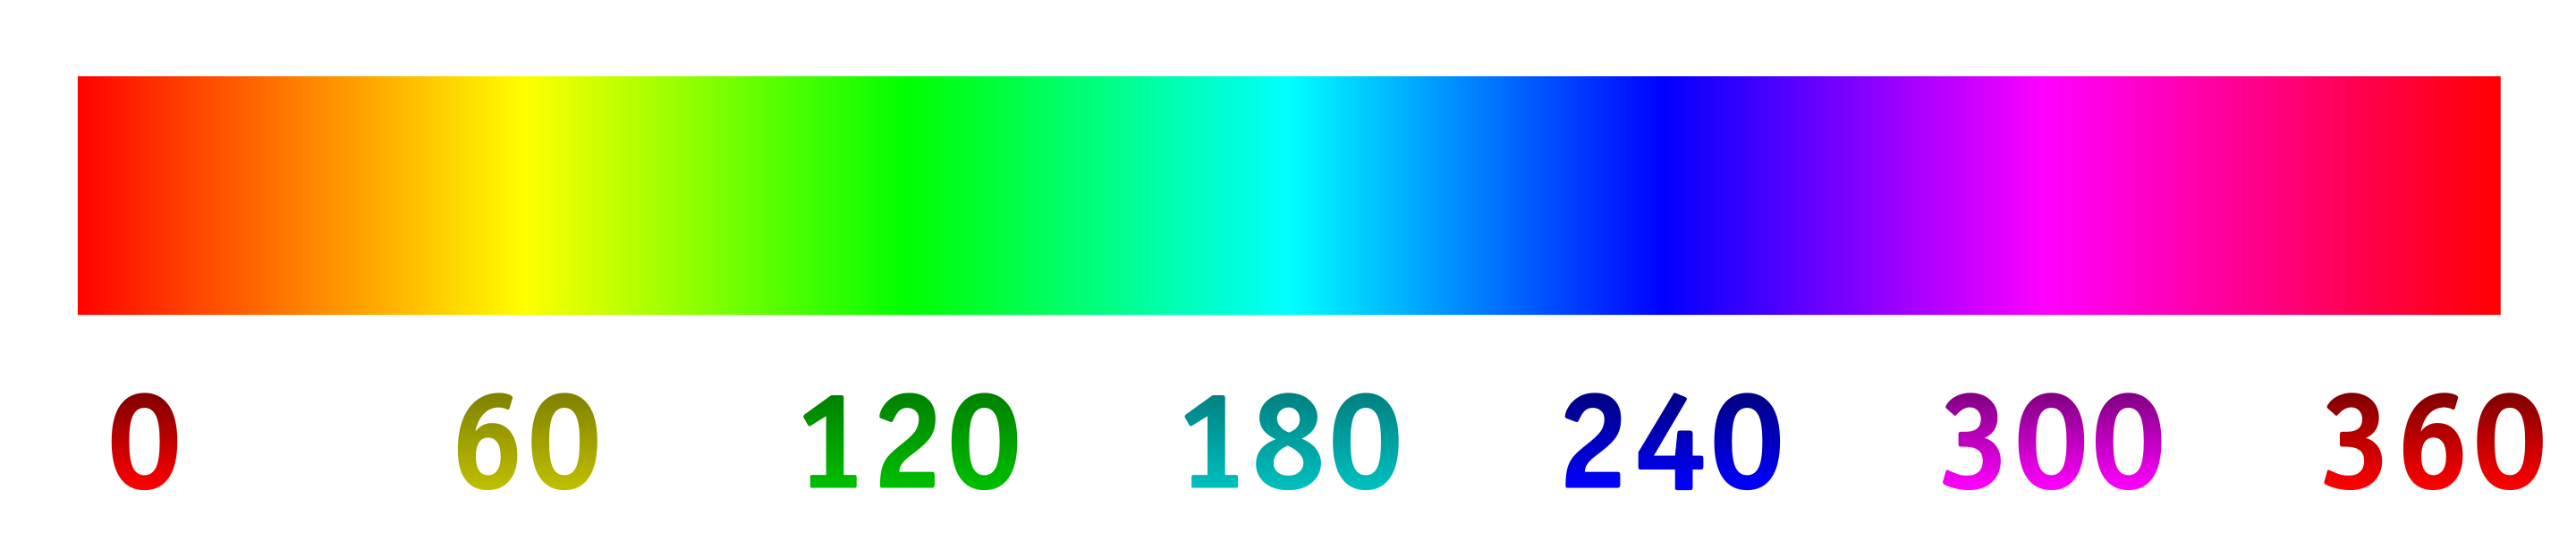
\includegraphics[width=7cm]{hue_scale.png}
    \caption{Barvy odpovídající úhlu H v HSV nebo HSL modelu \cite{wiki:Hue}.}
    \label{fig:huerotate-scale}
\end{figure}

Na obrázku \ref{fig:huerotate-res} jsou vidět aplikované inkrementy H o určitý úhel.
\begin{figure}[h]
    \centering
    \begin{subfigure}[t]{0.4\textwidth}
        \vskip 0pt
        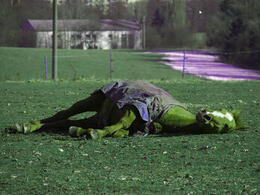
\includegraphics[width=1.0\textwidth]{horse_hue_60.jpg}
        \caption{$H + 60^\circ$}
    \end{subfigure}
    \hspace{1cm}
    \begin{subfigure}[t]{0.4\textwidth}
        \vskip 0pt
        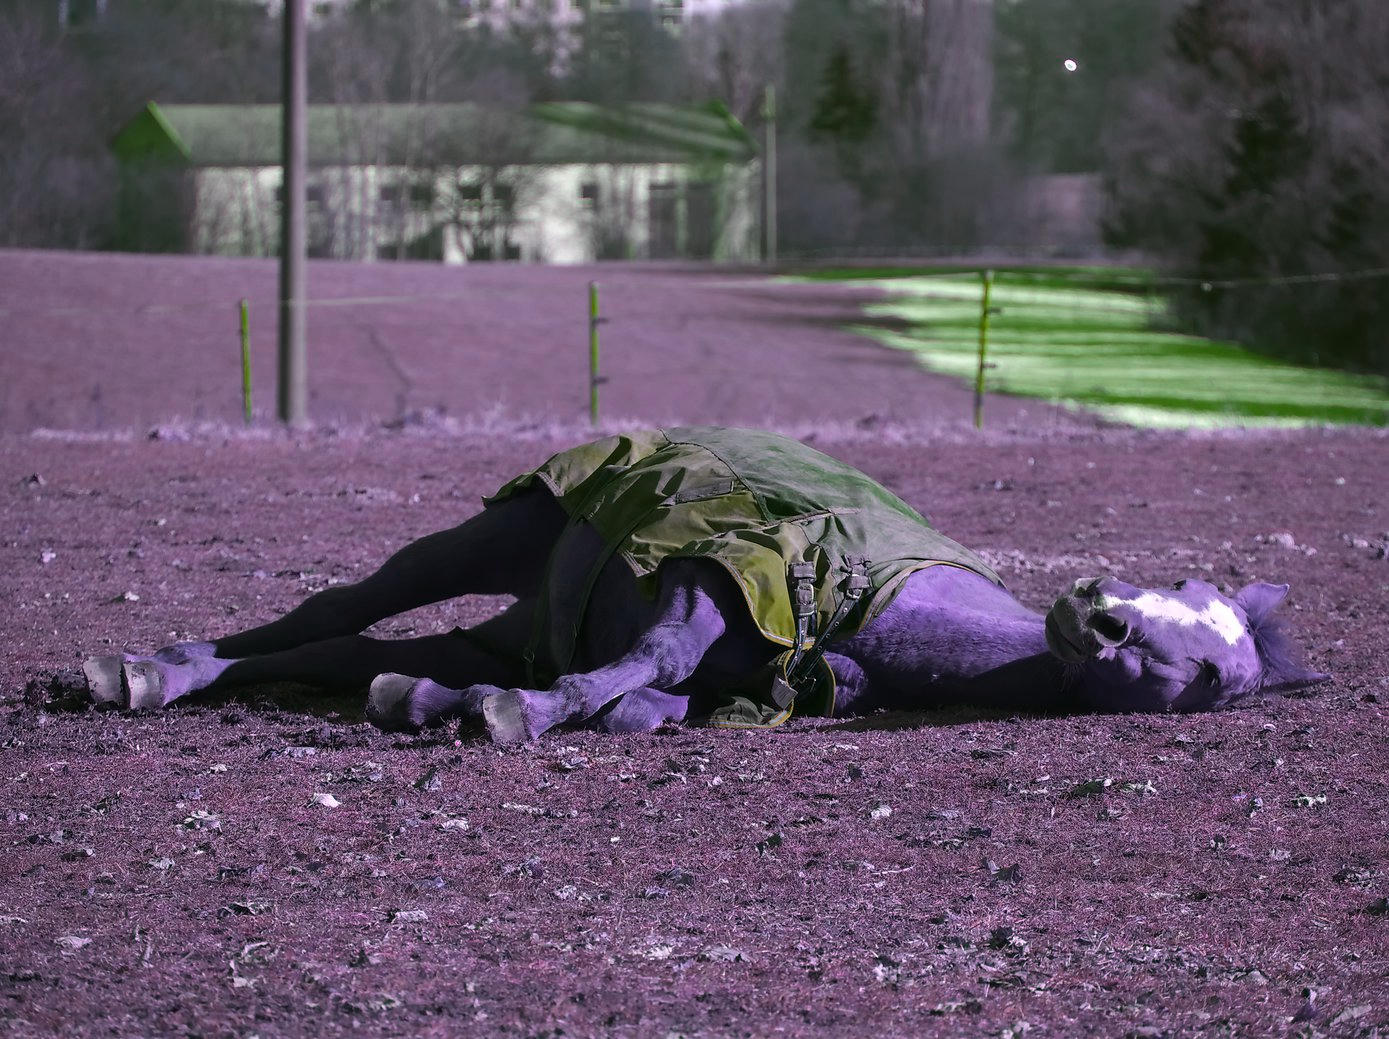
\includegraphics[width=1.0\textwidth]{horse_hue_240.jpg}
        \caption{$H + 240^\circ$}
    \end{subfigure}
    \caption{Ukázka rotace odstínu o určité úhly.}
    \label{fig:huerotate-res}
\end{figure}

\subsubsection{Vlastní operace zesvětlení}
Jelikož operace \uv{expozice} a \uv{gamma} nedávají moc pěkné výsledky.
Byla implementována vlastní formule, která se pokouší o zesvětlení a ztmavení obrazu při zachování vnímaného kontrastu.

Prvním pokusem bylo pro zvětšení barev použít násobení místo inkrementace.
Výsledek je vidět na obrázku \ref{fig:multiplication}.
\begin{figure}[h]
    \centering
    \begin{subfigure}[t]{0.24\textwidth}
        \vskip 0pt
        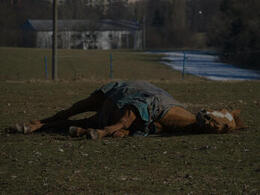
\includegraphics[width=1.0\textwidth]{horse_mul_down.jpg}
        \caption{$c = 0.5$}
    \end{subfigure}
    \begin{subfigure}[t]{0.24\textwidth}
        \vskip 0pt
        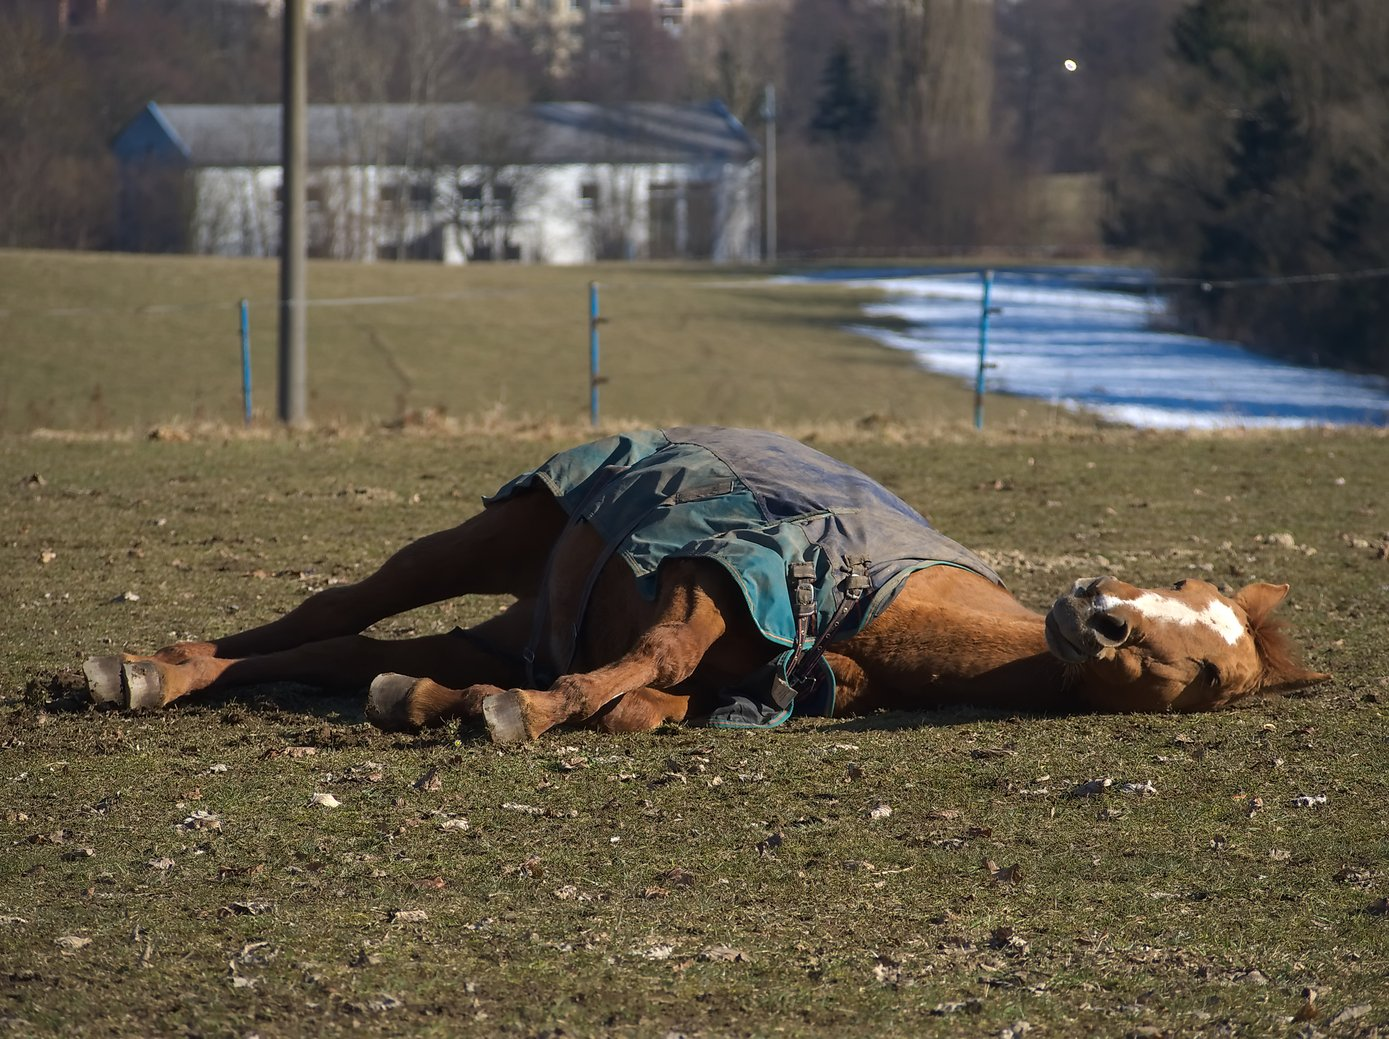
\includegraphics[width=1.0\textwidth]{horse_original.jpg}
        \caption{$c = 1$ -- původní}
    \end{subfigure}
    \begin{subfigure}[t]{0.24\textwidth}
        \vskip 0pt
        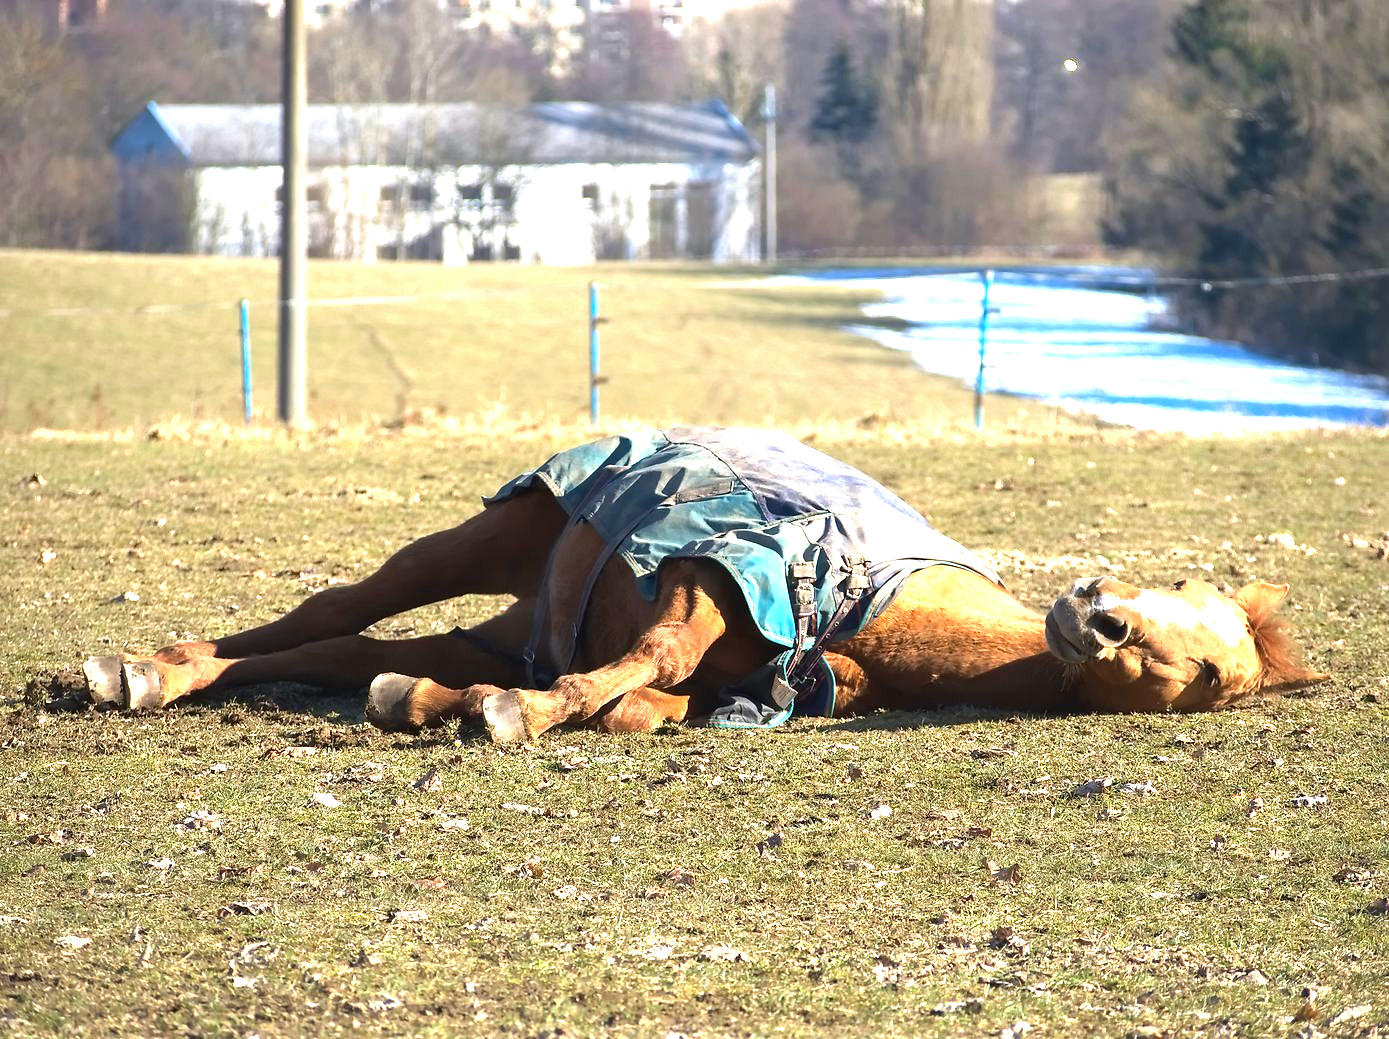
\includegraphics[width=1.0\textwidth]{horse_mul_up.jpg}
        \caption{$c = 2.0$}
    \end{subfigure}
    \begin{subfigure}[t]{0.24\textwidth}
        \vskip 0pt
        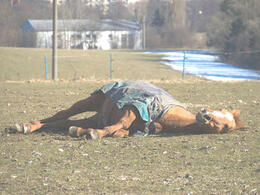
\includegraphics[width=1.0\textwidth]{horse_exposure_plus.jpg}
        \caption{Zesvětlení pomocí \uv{expozice} pro srovnání}
    \end{subfigure}
    \caption{Ztmavení a zesvětlení pomocí násobení skalární hodnotou $c$.}
    \label{fig:multiplication}
\end{figure}

Je vidět zlepšení vizuální kvality, kde kontrast neutrpěl změnu.
Lze si všimnout, že tmavé hodnoty nejsou ovlivněny tak moc jako světlé, které většinou velice rychle dosáhnou maximální hodnoty a tvoří přepaly.
Proto byla implementována formule s gamma korekcí, která nelineárně změní hodnotu násobícího koeficientu, tak aby byly více ovlivněny body tmavé a u světlých nedocházelo k přepalům.
Zde je formule:
$$P' = P\left(1 + (c - 1)(1 - L^{0.5})\right)$$
, kde:
\begin{itemize}
    \item $c > 1$ -- míra zesvětlení
    \item $L = 0,299R + 0,587G + 0.114B$ -- Světlost pixelu
\end{itemize}
Pro $c < 1$ se formule upraví na:
$$P' = P\left(1 - (1 - c)(1 - L^{1.5})\right)$$
což způsobí pomalejší úbytek  u světlejších bodů a rychlejší úbytek u bodů tmavších.
Na obrázku \ref{fig:multiplication-luma} je vidět finální výsledek na dvou různých obrázcích.
\begin{figure}[h]
    \centering
    \begin{subfigure}[t]{0.25\textwidth}
        \vskip 0pt
        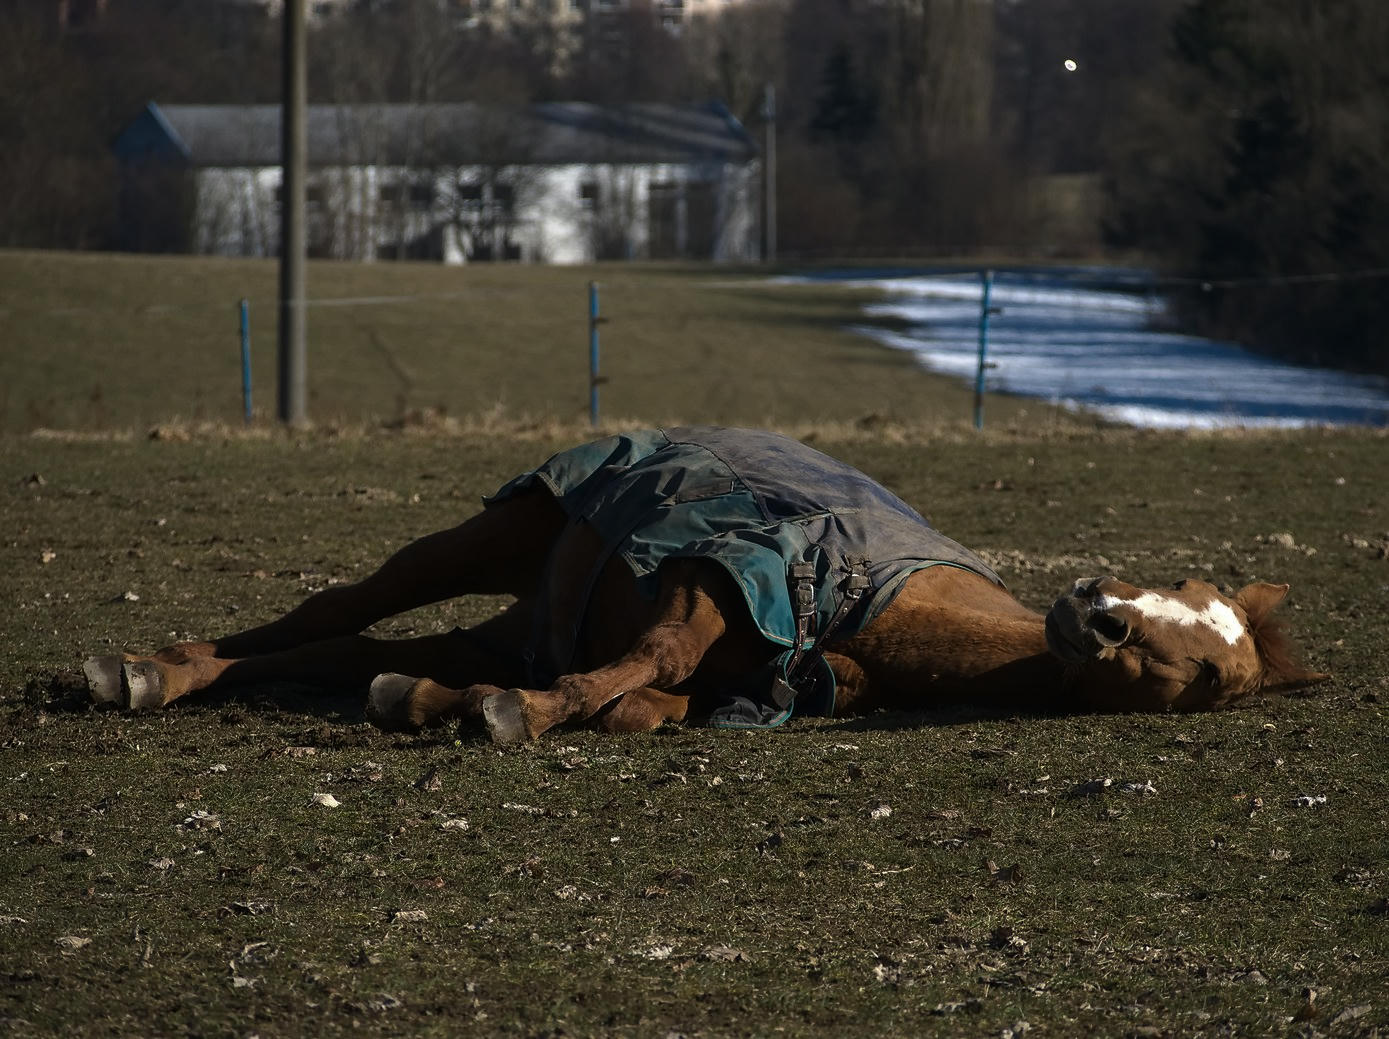
\includegraphics[width=1.0\textwidth]{horse_mul_luma_down.jpg}
        \caption{$c = 0.5$}
    \end{subfigure}
    \hspace{1cm}
    \begin{subfigure}[t]{0.25\textwidth}
        \vskip 0pt
        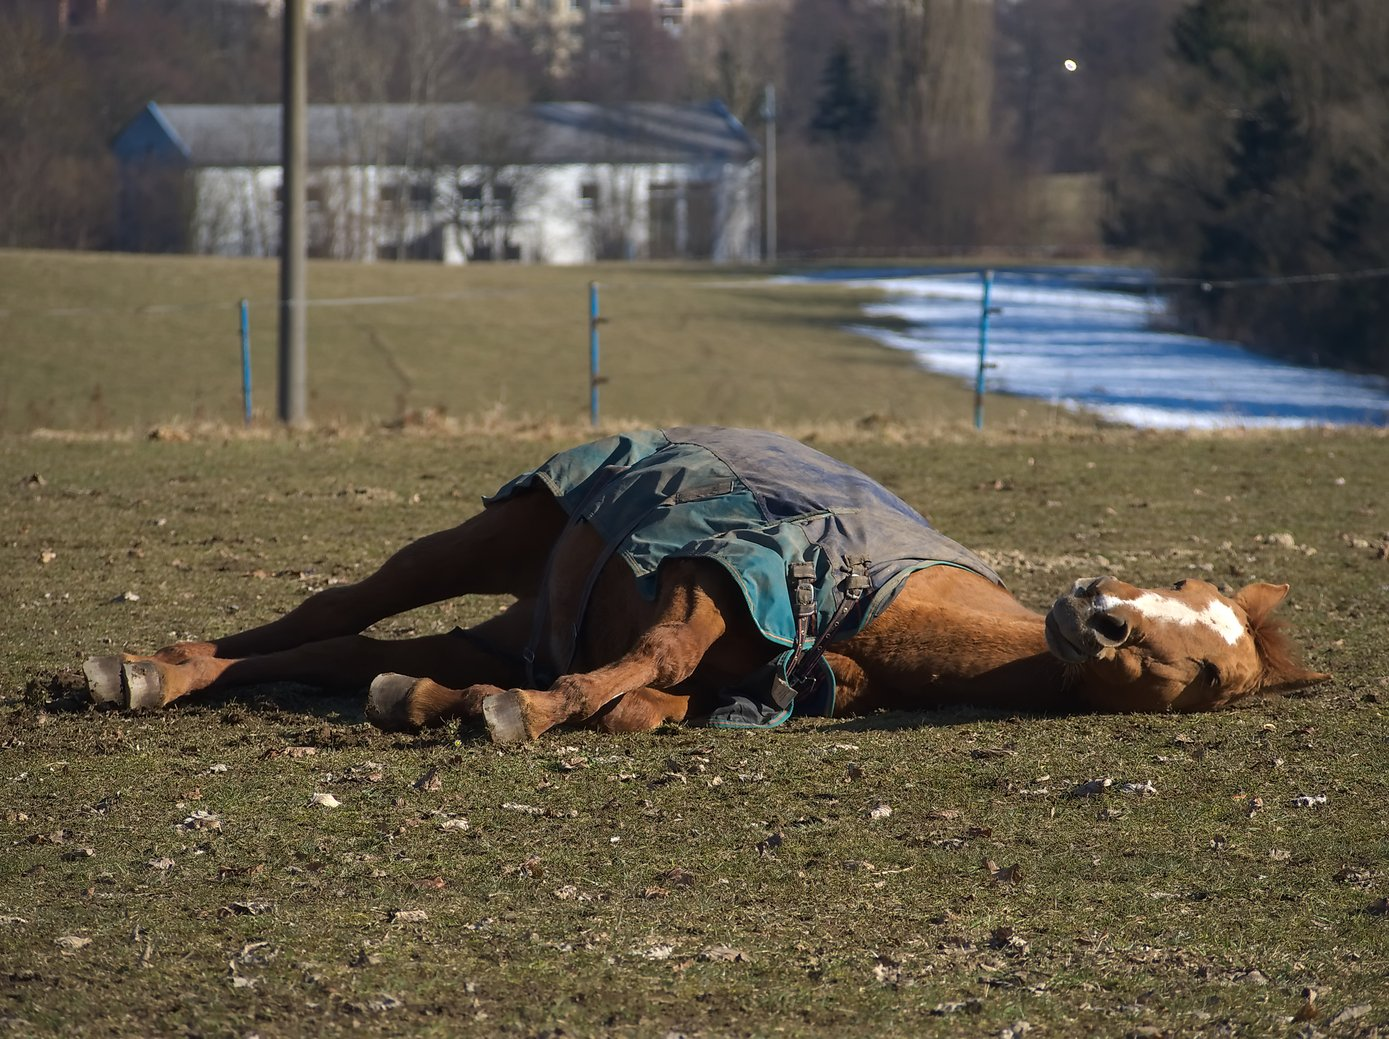
\includegraphics[width=1.0\textwidth]{horse_original.jpg}
        \caption{$c = 1$ -- původní}
    \end{subfigure}
    \hspace{1cm}
    \begin{subfigure}[t]{0.25\textwidth}
        \vskip 0pt
        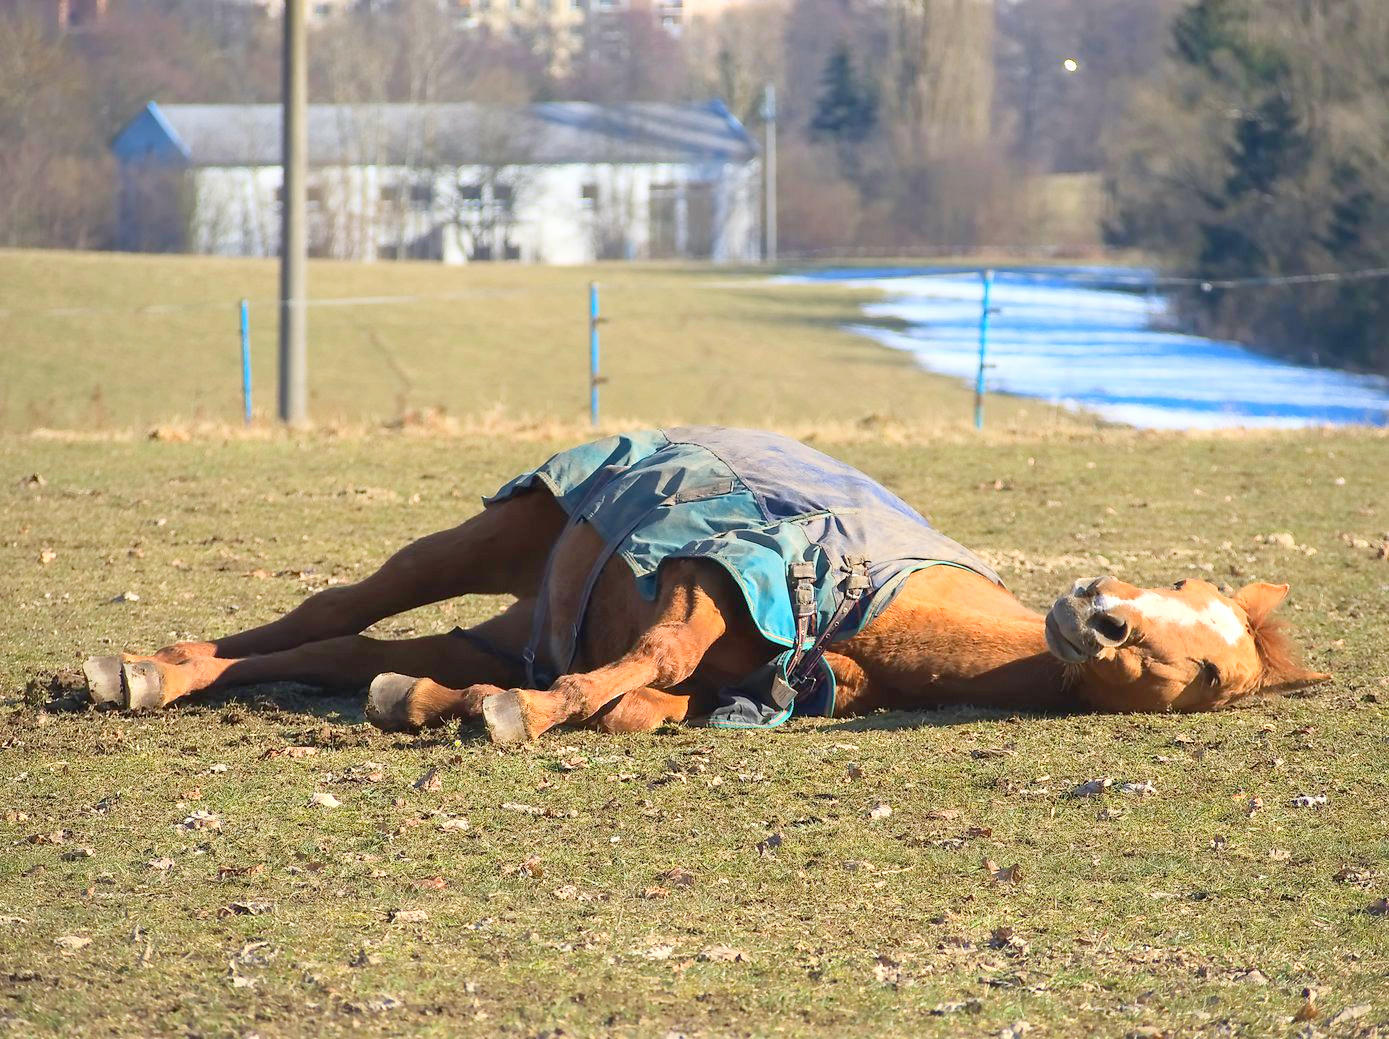
\includegraphics[width=1.0\textwidth]{horse_mul_luma_up.jpg}
        \caption{$c = 3.0$ -- Obrázek je znatelně světlejší ale nedochází k přepalům.}
    \end{subfigure}
    \begin{subfigure}[t]{0.25\textwidth}
        \vskip 0pt
        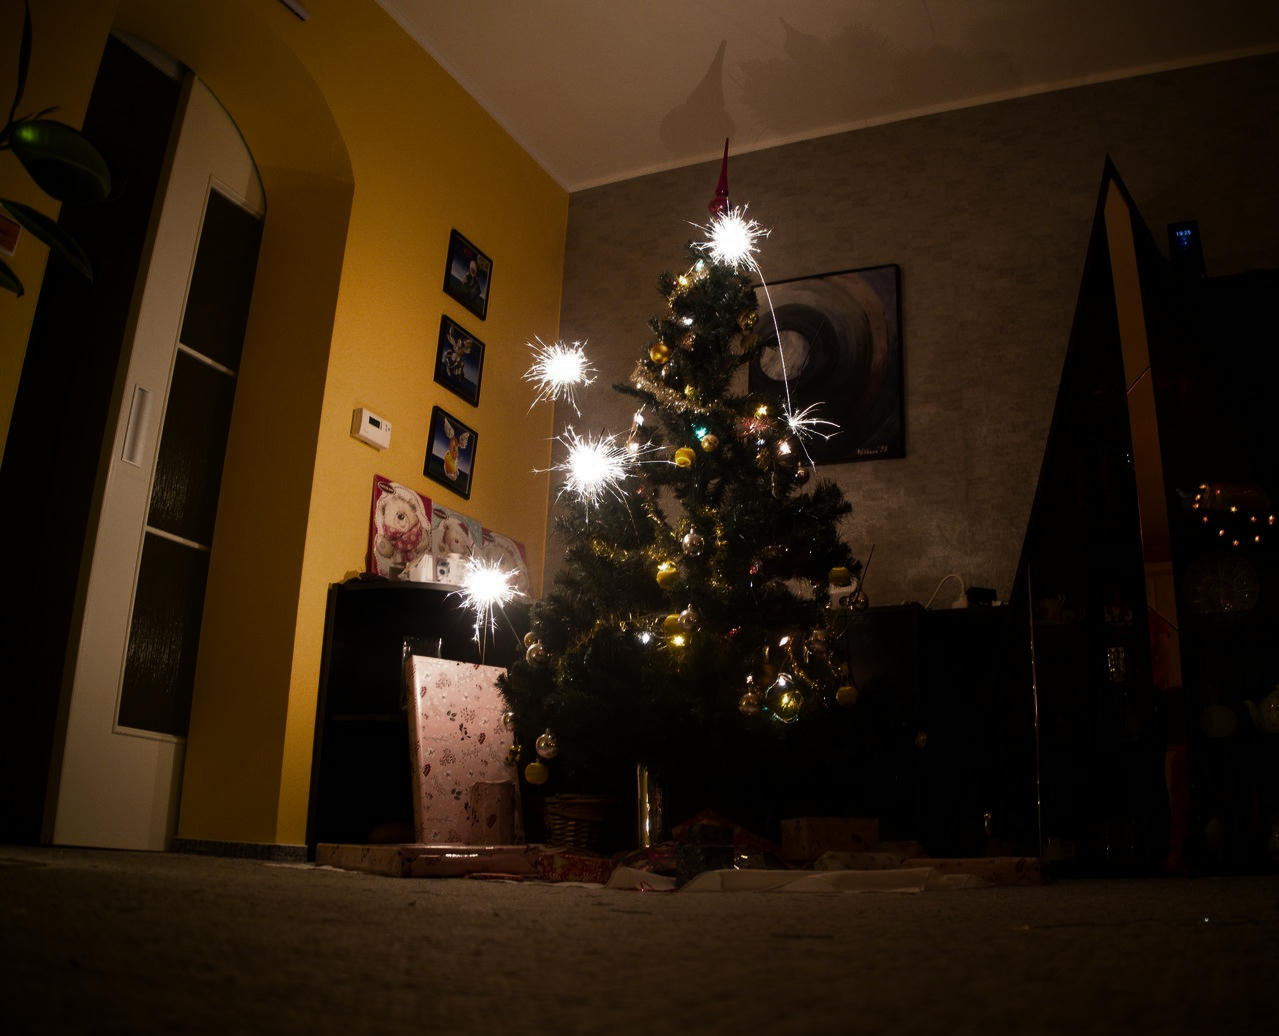
\includegraphics[width=1.0\textwidth]{tree_luma_mult_down.jpg}
        \caption{$c = 0.3$}
    \end{subfigure}
    \hspace{1cm}
    \begin{subfigure}[t]{0.25\textwidth}
        \vskip 0pt
        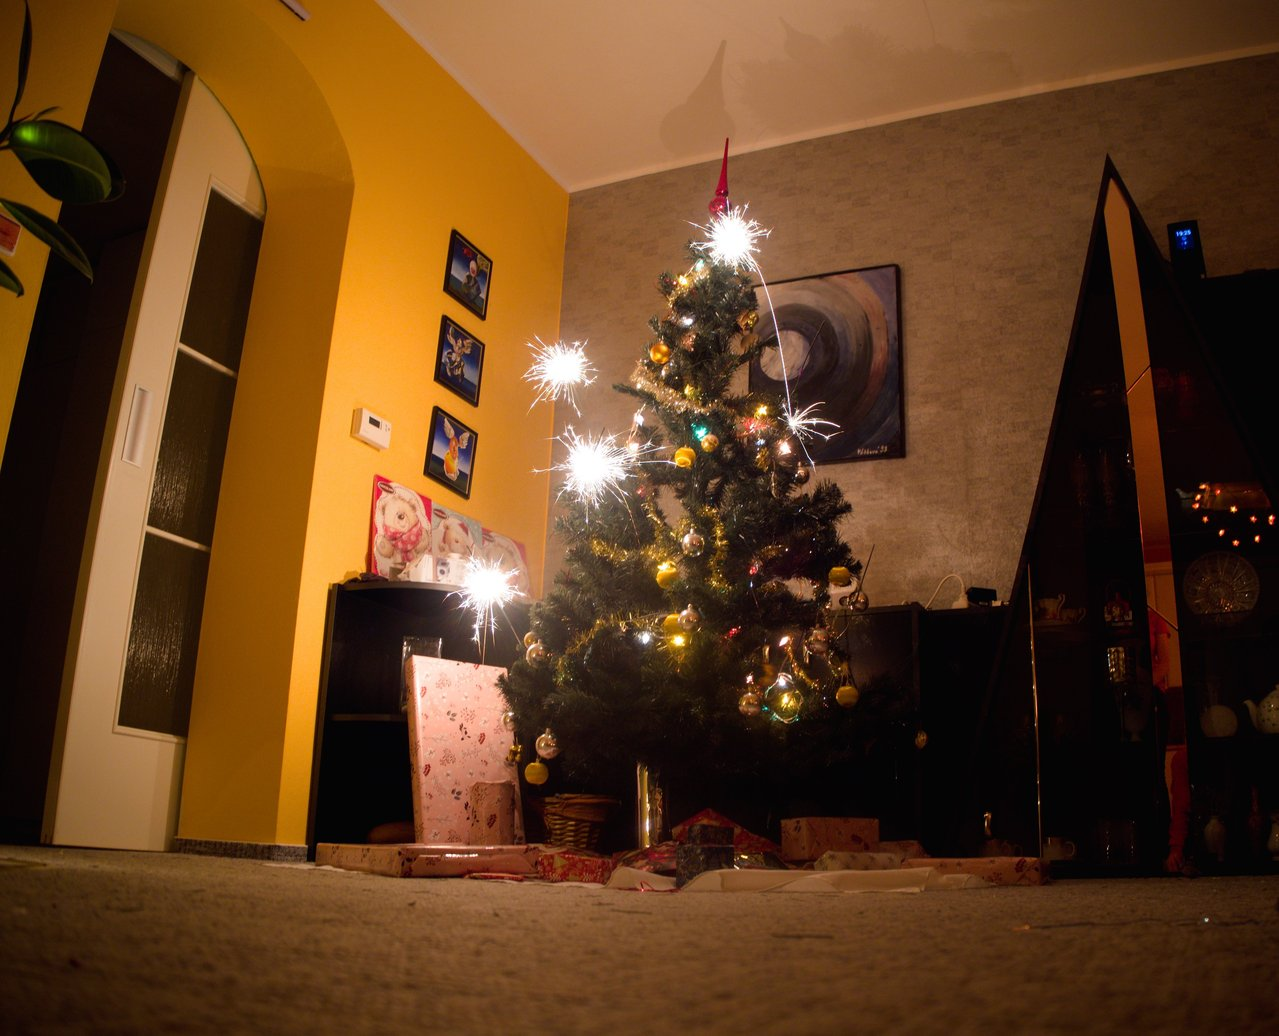
\includegraphics[width=1.0\textwidth]{tree_original.jpg}
        \caption{$c = 1$ -- původní}
    \end{subfigure}
    \hspace{1cm}
    \begin{subfigure}[t]{0.25\textwidth}
        \vskip 0pt
        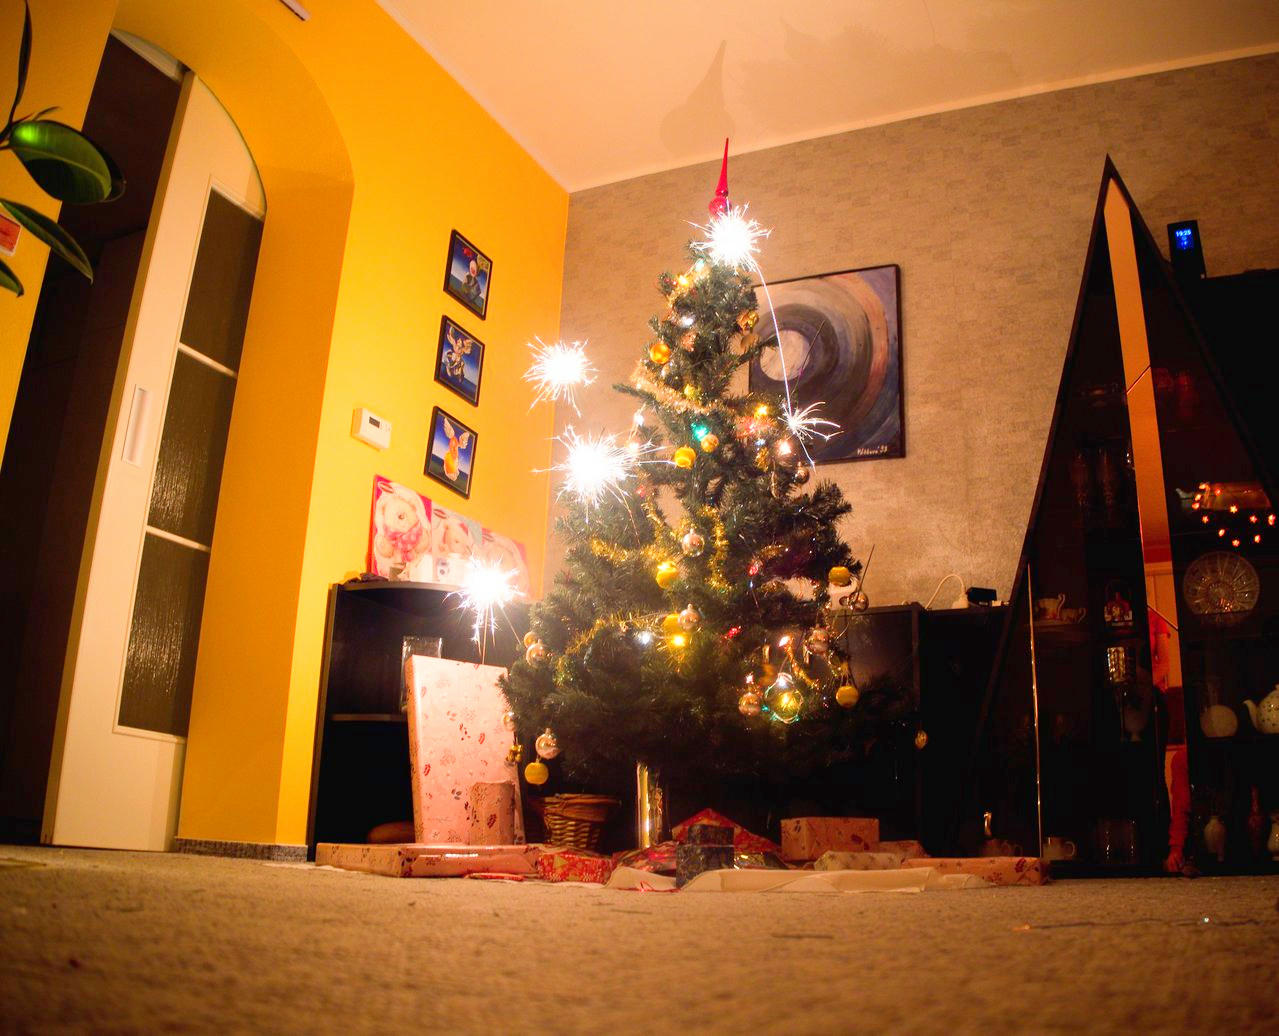
\includegraphics[width=1.0\textwidth]{tree_luma_mult_up.jpg}
        \caption{$c = 2.5$}
    \end{subfigure}
    \caption{Ztmavení a zesvětlení pomocí vlastní formule.}
    \label{fig:multiplication-luma}
\end{figure}

\subsection{Obecné barevné transformace a vlastní filtry}
Aplikace umožňuje nadefinovat vlastní transformaci barev:
$$
P'
=
\begin{bmatrix}
    A_r & A_g & A_b \\
    B_r & B_g & B_b \\
    C_r & C_g & C_b \\
\end{bmatrix}
\cdot
\begin{bmatrix}R\\G\\B\end{bmatrix}
$$
Kde $A_x$, $B_x$ a $C_x$ si lze libovolně navolit v intervalu $\langle0, 2\rangle$.
Díky tomuto lze například implementovat vlastní filtry.
Vísledek lze vidět na obrázku \ref{fig:custom-filters}.
\begin{figure}[h]
    \centering
    \begin{subfigure}[t]{0.3\textwidth}
        \centering
        \vskip 0pt
        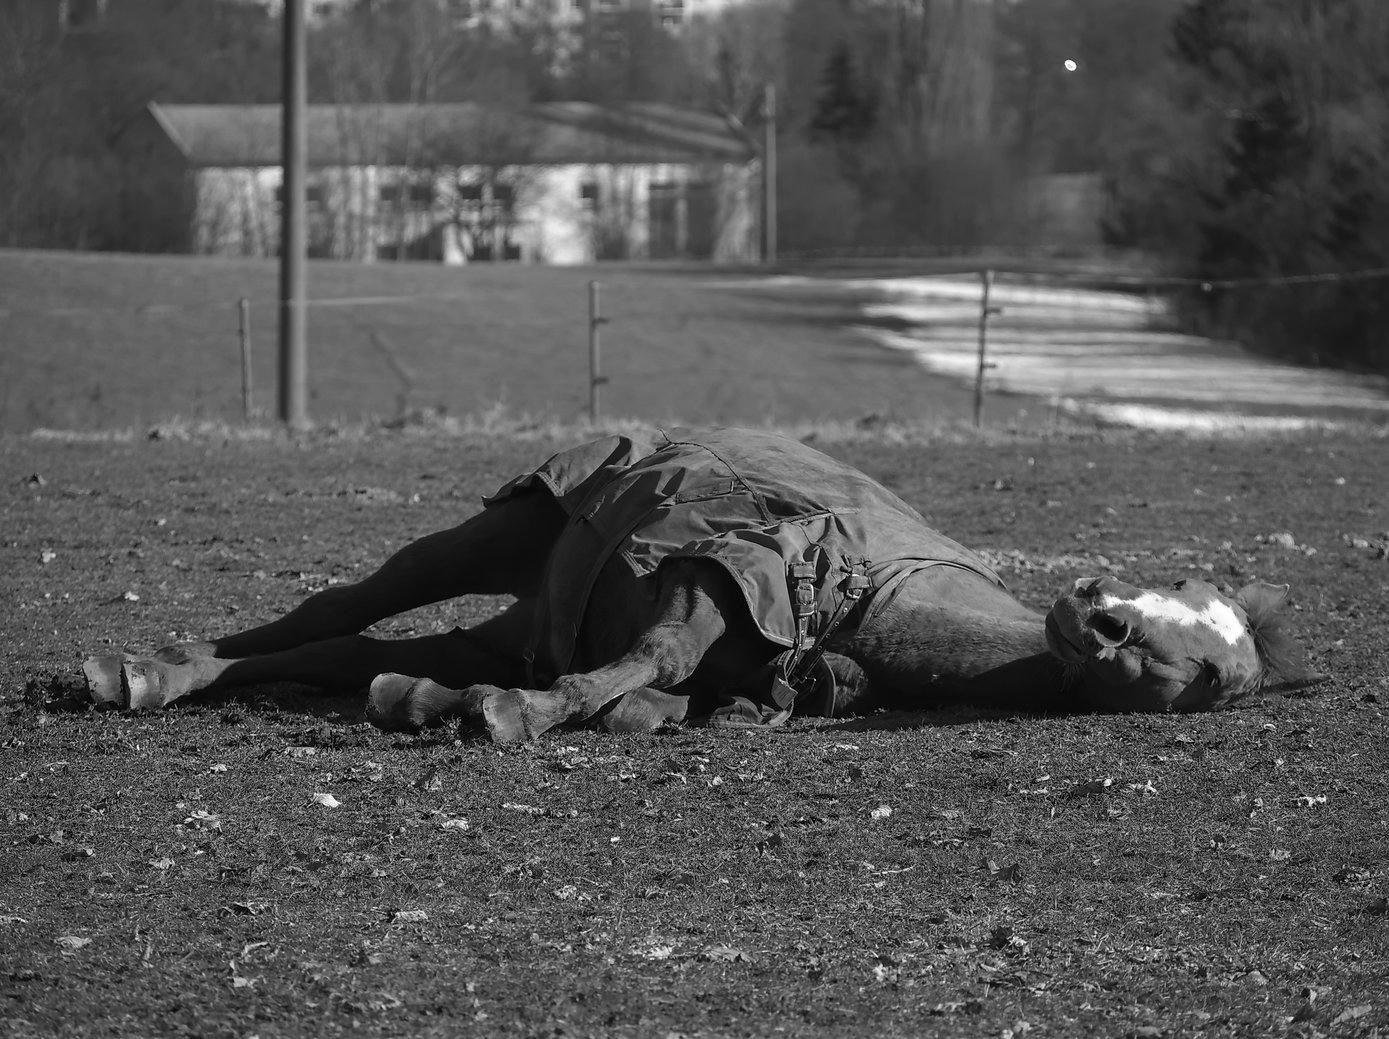
\includegraphics[width=0.8\textwidth]{horse_average.jpg}
        \caption{
        $
            \begin{bmatrix}
                1/3 & 1/3 & 1/3 \\
                1/3 & 1/3 & 1/3 \\
                1/3 & 1/3 & 1/3 \\
            \end{bmatrix}
            \cdot
            \begin{bmatrix}R\\G\\B\end{bmatrix}
        $\\\\Luma nekorektní černobílá
        }
    \end{subfigure}
    \hspace{0.1cm}
    \begin{subfigure}[t]{0.3\textwidth}
        \centering
        \vskip 0pt
        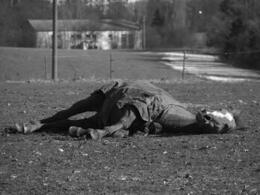
\includegraphics[width=0.8\textwidth]{horse_luma.jpg}
        \caption{
            $
            \begin{bmatrix}
                0,299 & 0,587 & 0,114 \\
                0,299 & 0,587 & 0,114 \\
                0,299 & 0,587 & 0,114 \\
            \end{bmatrix}
            \cdot
            \begin{bmatrix}R\\G\\B\end{bmatrix}
            $\\\\Luma korektní černobílá
        }
    \end{subfigure}
    \hspace{0.1cm}
    \begin{subfigure}[t]{0.3\textwidth}
        \centering
        \vskip 0pt
        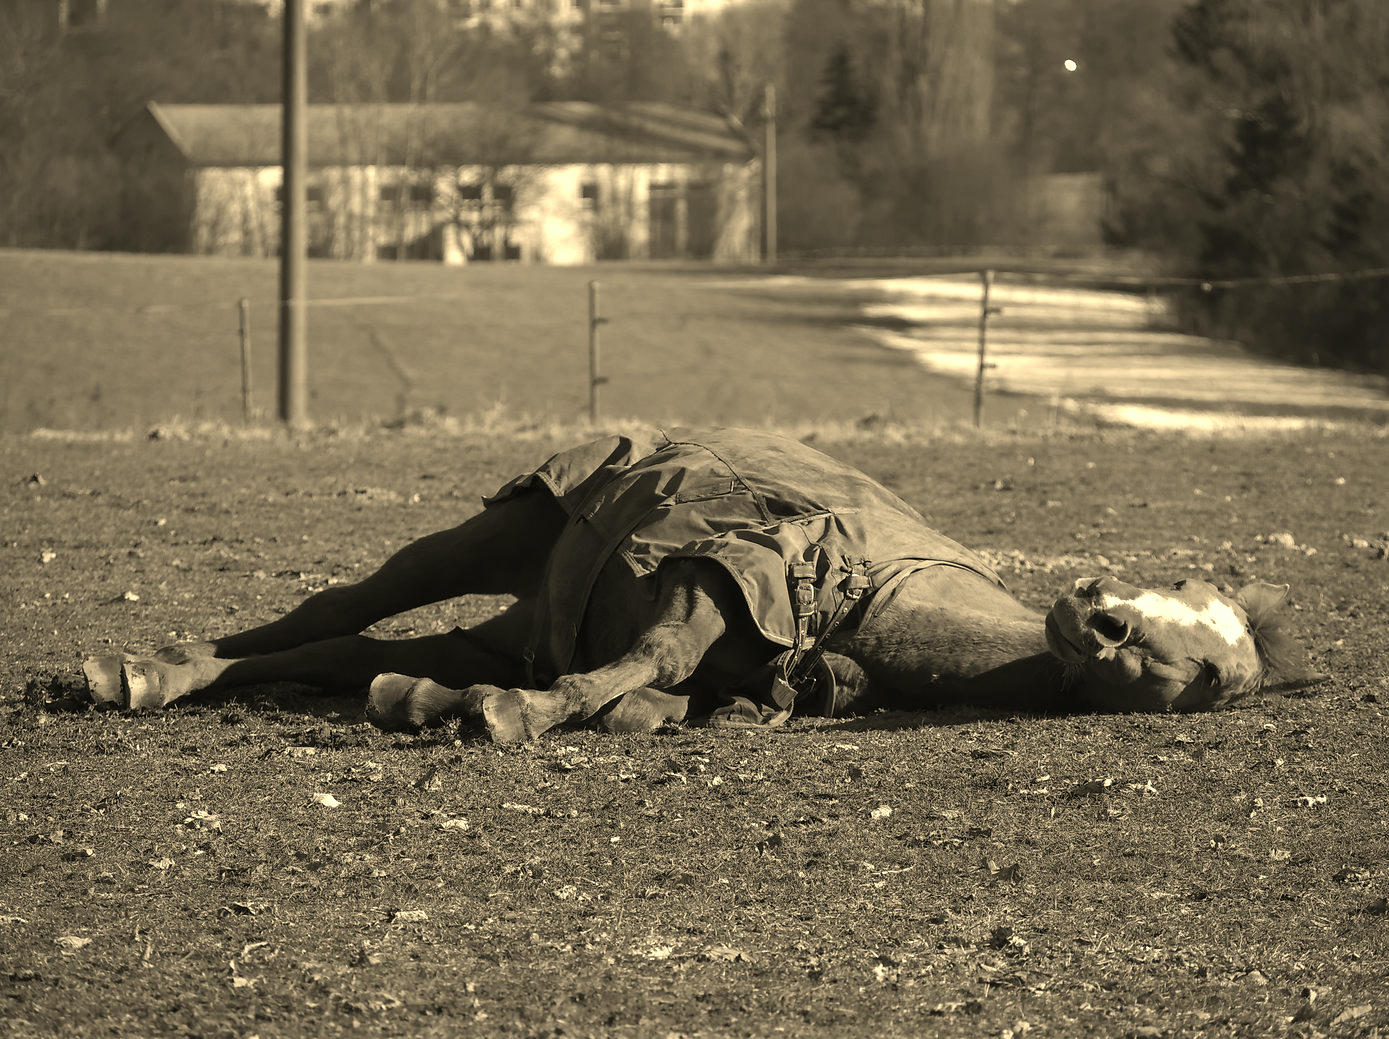
\includegraphics[width=0.8\textwidth]{horse_sepia.jpg}
        \caption{
            $
            \begin{bmatrix}
                0,393 & 0,769 & 0,189 \\
                0,349 & 0,686 & 0,168 \\
                0,272 & 0,534 & 0,131 \\
            \end{bmatrix}
            \cdot
            \begin{bmatrix}R\\G\\B\end{bmatrix}
            $\\\\Efekt \uv{sépie}\cite{Howtocon48:online}
        }
    \end{subfigure}
    \caption{Demonstrace příkladů vlastních filtrů.}
    \label{fig:custom-filters}
\end{figure}
Filtru lze také nastavit mírů aplikování, tedy lineární interpolaci mezi původním obrázkem a plně transformovaným.

\section{Závěr}
Tento projekt prozkoumal základní vlastnosti editorů a v rámci něj byla vytvořena aplikace, která demonstruje jak jednotlivé filtry fungují pomocí lineárních posuvníků.
Rovněž umožňuje vytvoření si vlastního filtru a následně jej použít, aby uživatel pochopil, jak se jednotlivé barvy v modelu RGB chovají.

\newpage

\bibliographystyle{alpha}
\begin{flushleft}
  \bibliography{project}
\end{flushleft}

%\appendix
%\newpage
%\section{}

\end{document}
